\chapter{Results}
\label{chap:resultados}

In this chapter, we present the results of the methodology steps. We present both process results as also the data and discussions of each method. Section \ref{sec:results-slr} shows the process results, as for withdrawing paper process. Section \ref{sec:results-theory} explains the Systematic Literature Review process. Section \ref{sec:results-gt} shows the process results. The next sections are focused on the three categories of data acquired and analyzed from both Systematic Literature Review and Grounded Theory. The categories are \textit{(i)} General (Section \ref{sec:results-general}), \textit{(ii)} Research (Section \ref{sec:results-research}), and \textit{(iii)} Empirical (Section \ref{sec:results-empirical}). Finally, Section \ref{sec:results-theory} presents all concepts related to a theory of Cognitive Impact Evaluation for people who are blind.

\section{Systematic Literature Review Results}
\label{sec:results-slr}
We have performed the search, selection and data extraction from the initial systematic literature review process and the snowballing process (forward and backward snowballing). The systematic literature review had four filters for both the initial and the snowballing processes. Appendix \ref{ap:A} details the complete list of selected papers and the spreadsheet\footnote{\url{https://www.dropbox.com/s/dvvn44cymqsqguy/Systematic\%20Review\%20-\%20Mesquita\%20L.\%202018.xlsm?dl=0}} has all data documented. Next, we present the results about the process: papers selected, papers withdrawn and the rates of acceptance.

Figure \ref{fig:filters_in_systematic_review_process} resumes the conducting phase results. The initial search brings us 2173 papers, among them, after the whole process, it remains 23 papers. Further, the snowballing process brings 690 papers (287 from forwarding snowballing and 403 backward snowballing), among them it remains 24 papers (15 from forwarding snowballing and 9 from backward snowballing). Then, at the final process of systematic literature review, we have 47 papers (23 from initial search and 24 from snowballing search). 

 	\begin{figure}[h] 
   	    \captionsetup{width=16cm}%Da mesma largura que a figura
		\Caption{\label{fig:filters_in_systematic_review_process} Filters in the Systematic Review Process}
		\UFCfig{}{
			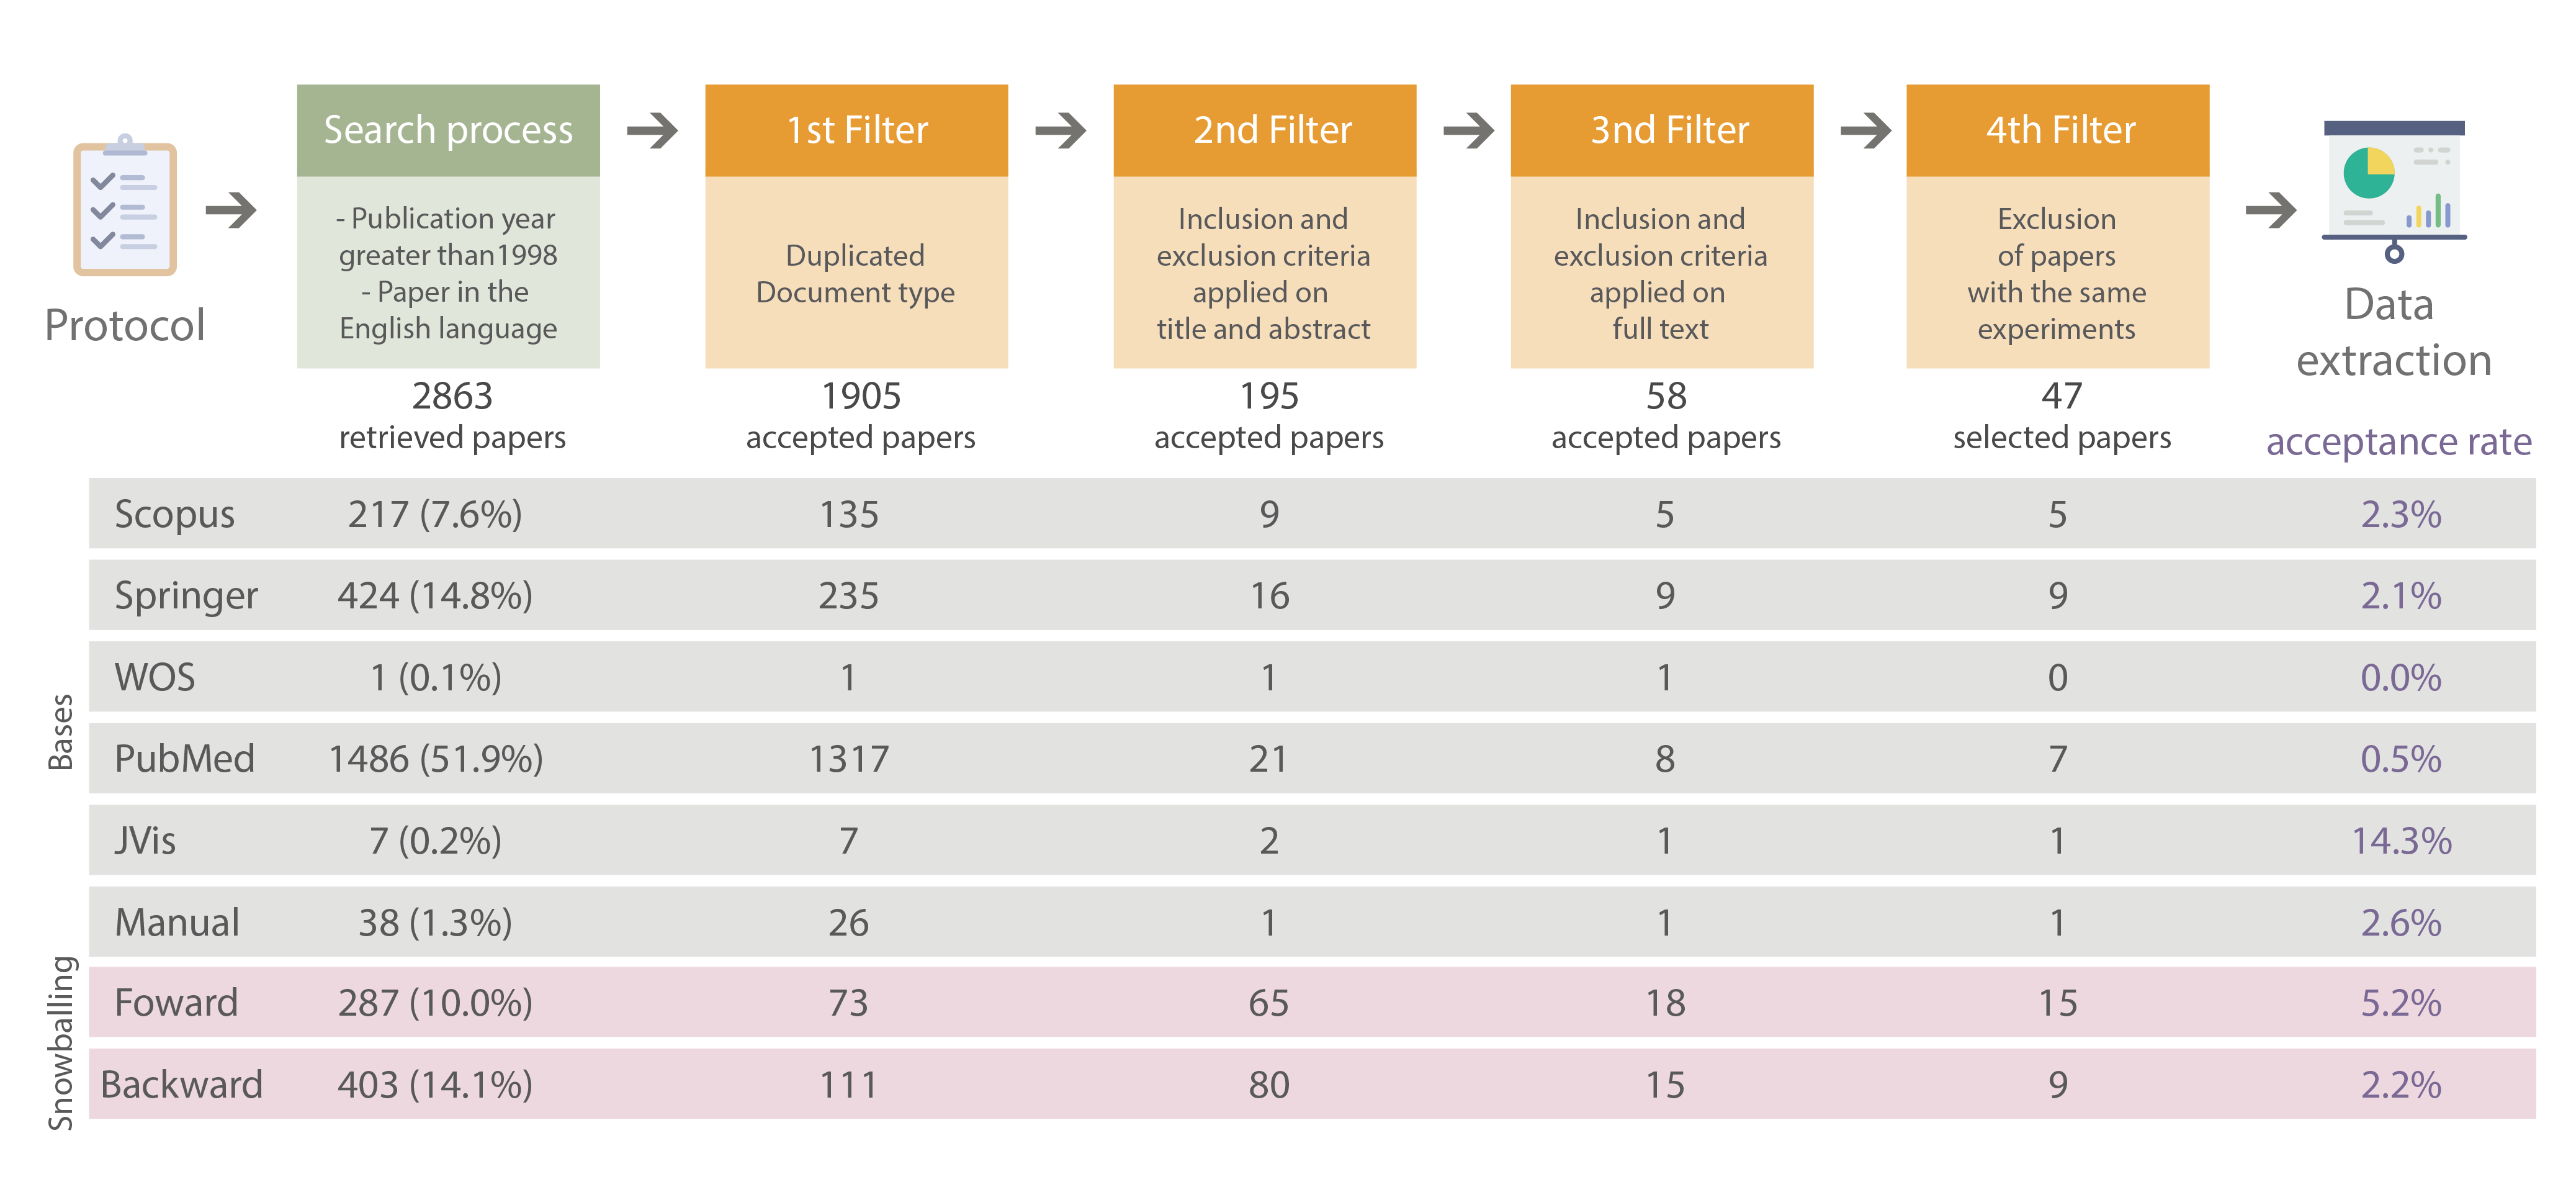
\includegraphics[width=16cm]{figuras/filters_in_systematic_review_process.png}
		}{
			\Fonte{Produced by the author.}
		}	
	\end{figure}

Regarding the acceptance rate (last column of Figure 1), the most important source for this search is the Visual Impairment \& Blindness Journal (\gls{JVis}). The acceptance rate of \gls{JVis} is 14.3\%, which means the number of accepted papers (1 paper) over the number of papers initially retrieved (7 papers). This rate is due to the journal's central theme is the subject sought in this review. Also, we can see that the snowballing process was a good step for the process since it had a large acceptance rate and a large number of papers selected.

Table \ref{tab:Acceptance of papers in_each_filter} shows the acceptance rate of each filter comparing with the last filter, e.g., the acceptance of forwarding snowballing papers in the third filter comparing to the papers selected on the second filter is 27.7\%. In this graph, the snowballing results again stand out. In the second filter, which filters by reading the abstract of the paper, we have an efficient selection with 72.1\% and 89.0\% for backward and forward respectively. These rates reinforce the significance of snowballing in the process.

\begin{table}[h]
	\captionsetup{width=11cm}%Deixe da mesma largura que a tabela
	\Caption{\label{tab:Acceptance of papers in_each_filter} Acceptance of papers in each filter}%
	\IBGEtab{}{%
		\begin{tabular}{m{2cm}m{2cm}m{2cm}m{2cm}m{1cm}}
			\toprule
			 & Total without snowballing & Backward snowballing & Forwarding snowballing & \textbf{Total}\\
			\midrule \midrule
			\textbf{First filter} & 79.2\% & 27.5\% & 25.4\% & \textbf{66.5\%} \\
			\textbf{Second filter} & 2.9\% & 72.1\% & 89.0\% & \textbf{10.2\%} \\
			\textbf{Third filter} & 50.0\% & 18.8\% & 27.7\% & \textbf{29.7\%} \\     
			\textbf{Fourth filter} & 92.0\% & 60.0\% & 83.3\% & \textbf{81.0\%} \\
			\bottomrule
		\end{tabular}%
	}{%
	\Fonte{Produced by the author.}%
%	\Nota{esta é uma nota, que diz que os dados são baseados na	regressão linear.}%
%	\Nota[Anotações]{uma anotação adicional, seguida de várias outras.}%
    }
    \end{table}

To better understand the snowballing process, we track from where each paper came from and how many papers were accepted of each one. Figure \ref{fig:snowballing_acceptance} shows how many papers brings each paper selected in the initial process and how many of them had been selected. We highlight two papers: ``A Virtual Environment for People Who Are Blind – A Usability Study'' \cite{201219} and ``Assessment of Indoor Route-finding Technology for People with Visual Impairment'' \cite{20105}.

 	\begin{figure}[h] 
   	    \captionsetup{width=16cm}%Da mesma largura que a figura
		\Caption{\label{fig:snowballing_acceptance} Snowballing process}
		\UFCfig{}{
			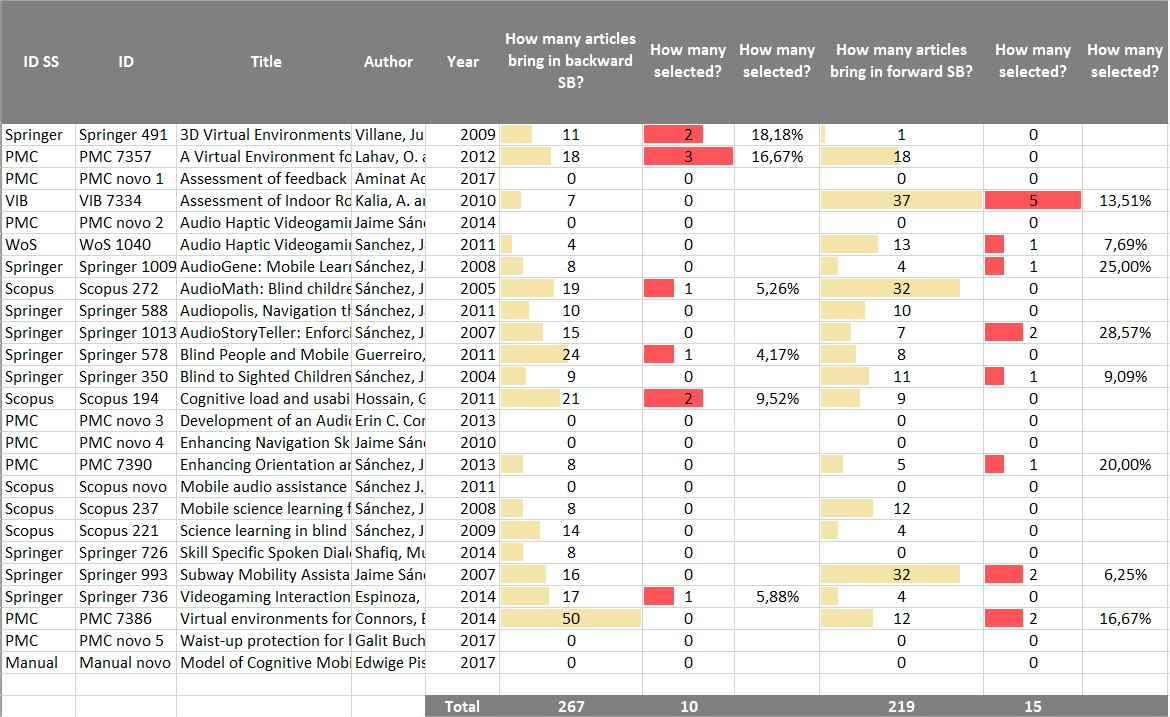
\includegraphics[width=16cm]{figuras/snowballing_acceptance.jpg}
		}{
			\Fonte{Produced by the author.}
		}	
	\end{figure}

\subsection{Withdrawn papers}
\label{subsec:results-slr-withdrawal-papers}

Many papers excluded in the first filter are from the scientific base PubMed Central (\gls{PMC}), this is due to a lot of medical papers focused on disease effectiveness and specific medical statements. Even though the area of this study is computer science, we decided to insert the \gls{PMC} in the bases’ list due to the nature of the subject. To help the exclusion process, we highlighted some keywords not desired in the titles, like ``malaria'' or ``Alzheimer'', which facilitates the exclusion. 

Figure \ref{fig:reasons_for_withdrawn_pappers} shows the reasons for withdrawing papers in the third filter regarding the whole paper and the inclusion criteria. The main reason for withdrawing a paper in the last filter was ``the paper’s evaluation is out the search'' (105 papers excluded), which mainly consider the evaluation focused on the system performance and not on the user cognitive impact assessment. The other reasons are: 
        \begin{enumerate}
            \item The experiment not described in the paper (3 papers);
            \item The paper was not available to download from our online library's catalog of holdings or open access journals (6 papers);
            \item The system is not according to the inclusion criteria (8 papers);
            \item The paper is a Solution Proposal \cite{Petersen2008} focused on, for example, a model or a framework with or without evaluation (4 papers);
            \item The paper is a Philosophical Paper \cite{Petersen2008} (11 papers), e.g., reviews. 
        \end{enumerate}

 	\begin{figure}[h] 
   	    \captionsetup{width=12cm}%Da mesma largura que a figura
		\Caption{\label{fig:reasons_for_withdrawn_pappers} Reasons for paper withdrawn}
		%TODO alterar na figura!
		\UFCfig{}{
			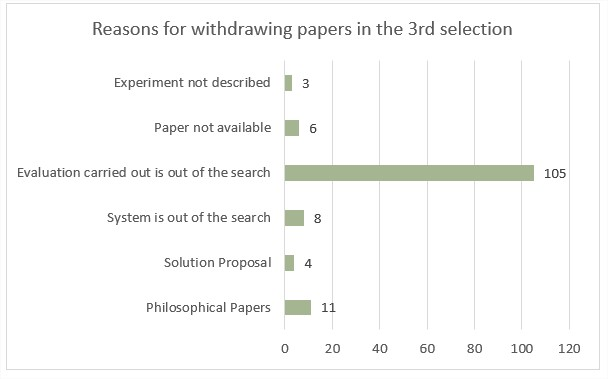
\includegraphics[width=12cm]{figuras/reasons_for_withdrawn_pappers.jpg}
		}{
			\Fonte{Produced by the author.}
		}	
	\end{figure}

% \subsection{Cross Validation}
% \label{subsec:results-slr-cross-validation}

% To reduce the bias, we apply a cross-validation on the third filter selection of the systematic literature review, on which we read the entire papers to select them, regarding the inclusion criteria. We use the selection result to compare with our and to get the accuracy of the filter. We send the quality form to five specialists on HCI themes. We send a list of 20 papers and we expect they validate a sort of 10 papers. 

% At final, two specialists answered, and the accuracy obtained was 59.2\% when comparing the selections of specialists and our selection. Figure \ref{fig:cross_validation} shows the results obtained of each expert. Due to the low rate of answers, we analyze each paper and its reason to withdraw case-by-case. After removing the papers with conflict (one expert accept and the other reject) and the papers with only one answer, we obtained an accuracy of 75.0\%.


%     \begin{figure}[h] 
%   	    \captionsetup{width=12cm}%Da mesma largura que a figura
% 		\Caption{\label{fig:cross_validation_results} Cross-validation Results}
% 		%TODO alterar na figura!
% 		\UFCfig{}{
% 			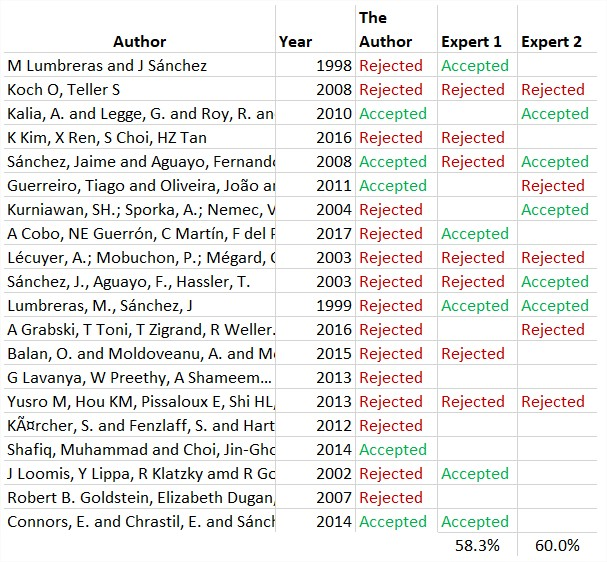
\includegraphics[width=12cm]{figuras/cross_validation_results.jpg}
% 		}{
% 			\Fonte{Produced by the author.}
% 		}	
% 	\end{figure}

\section{Grounded Theory results}
\label{sec:results-gt}
The Grounded Theory analysis was performed to enhance and strengthen the findings of the Systematic Literature Review regarding cognitive evaluation concepts used in the context of this search, multimodal interfaces for people who are blind. The data used came from the systematic literature review process. 

In Grounded Theory, we use the method to analyses in detail four items from Empirical category: Hypothesis, Variables, Measures, and Tasks. The final map produced by the Selective Coding phase (explained in the Section \ref{sec:methodology-gt}) represents the main idea of the cognitive evaluation in the context of this study and connect all elements. This map is the main input to create the Guidelines.

%%%% Comentário do .doc%%%%
%Esse parágrafo foi feito na tentativa de mesclar os resultados e tinha colocado na introdução do capítulo. Porque se dividirmos m resultados da Revi. Sist. e do Ground Theory a categoria de Dados Empíricos será separada. Tanto que já explico na sessão Empirial Data (da Revisão sistemática) quais dados serão analisados por qual método. 

%Se mantiver separado é só desconsiderar este parágrafo.

In the Selective Coding, other elements of cognitive evaluation were mapped in the MAXQDA software to produce the map, as Sample and Ethical Concepts. For this reason, both systematic literature review and grounded theory results are present together in the Empirical section (Section \ref{sec:results-empirical}). The map of central idea is most explored in the Section \ref{sec:results-theory}.

Next, we will explain the data acquired from systematic literature review in the three categories: \textit{(i)} General, \textit{(ii)} Research, and \textit{(iii)} Empirical.

\section{General Results}
\label{sec:results-general}

Despite we consider as the final result of the systematic literature review the papers selected in the fourth filter, in this analysis of general data, we consider the 58 papers selected in the third filter. The type of data used in this category refers to papers within the search criteria. Therefore, it does not need to remove the papers that have cognitive experiments, even if papers have repeated experiments (kind of papers excluded in filter 4).

Regarding the empirical method, almost all papers use an Experiment as an empirical method (21 papers). Only 1 paper present a Case Study as an evaluation, that justifies the choice due to the small number of participants \cite{Sanchez2008}. This information was encountered in the text explicit or it was deducted from the details presented.

Figure \ref{fig:publication_year_of_papers} shows the papers selected regarding the timeline that starts in 2000 and has peaked in 2011 and 2014. These papers, published in the last years, give a comprehensive and valid picture of the existing evidence \cite{Wohlin2000}, considering that both the identification, the analysis, and the interpretation had conducted in a scientifically and rigorous way.

 	\begin{figure}[h] 
   	    \captionsetup{width=16cm}%Da mesma largura que a figura
		\Caption{\label{fig:publication_year_of_papers} Publication year of papers}
		\UFCfig{}{
			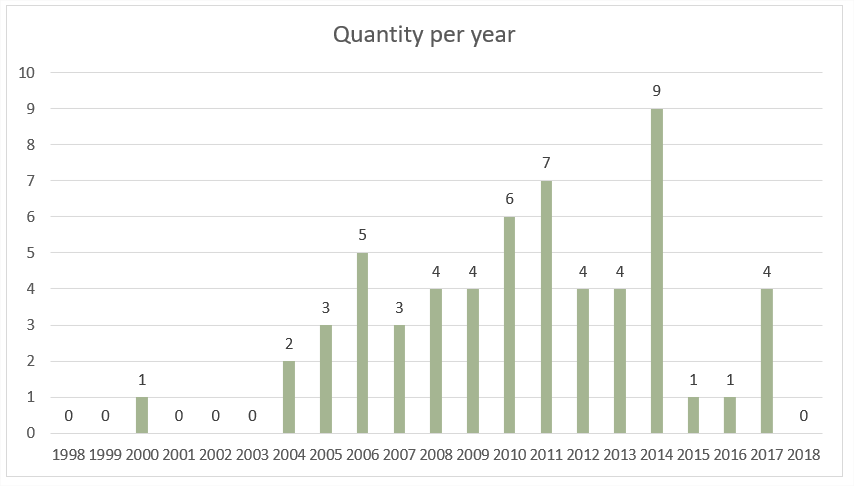
\includegraphics[width=16cm]{figuras/publication_year_of_papers.png}
		}{
			\Fonte{Produced by the author.}
		}	
	\end{figure}
	
\subsection{Qualitative evaluation}
\label{subsec:results-slr-qualitative-evaluation}

Each paper was evaluated according to the 8 questions of the quality form described in Section \ref{subsubsec:conducting-quality} and over again presented in the list below.

\begin{itemize}
    \item \textbf{Q1} Was it possible to extract all data regarding the data the Key features in multimodal interfaces (Classification category from extraction form? (-0.1 pt per missing input; min value: -4.1 pts)
    \item \textbf{Q2} Is there a complete description of how the evaluation has been applied? (1.0 pt per complete input in Empirical category; max value: 8,0 pts)
    \item \textbf{Q3} Are the groups of participants in the experiment randomly assigned? (0.5 pt)
    \item \textbf{Q4} Is the description of the impact evaluation understandable? (0.5 pt)
    \item \textbf{Q5} Does the article present different evaluation types of the proposal? (1 pt)
    \item \textbf{Q6} How many experiments does the paper present? (0.5 pt per experiment, if more than two experiments)
    \item \textbf{Q7} Is the goal of the evaluation cleared defined? (0.5 pt)
    \item \textbf{Q8} Is the hypothesis (null and alternative) explicitly described in the study? (0,5 pt)
\end{itemize}


The results of quality form range from 52\% to 96\% of expected quality, with average of 74\%. The expected quality means the maximum points in each question. We investigated the relationship between the quality score for each paper and both the date when the paper was published. The average quality scores for studies each year is shown in Figure \ref{fig:quality_form_of_papers}.

The quality points were not compared with the impact factor of journals or quality indexes of conferences, as CAPES index quality, and of journals, as h-index. The papers retrieved are from both conferences and journals which already includes the difficulty of comparison. Moreover, some journals and conferences have no index value, or they have different indexes, that also add problems to compare. Then we decided to do not cross this data.

 	\begin{figure}[h] 
   	    \captionsetup{width=16cm}%Da mesma largura que a figura
		\Caption{\label{fig:quality_form_of_papers} Quality form of papers}
		\UFCfig{}{
			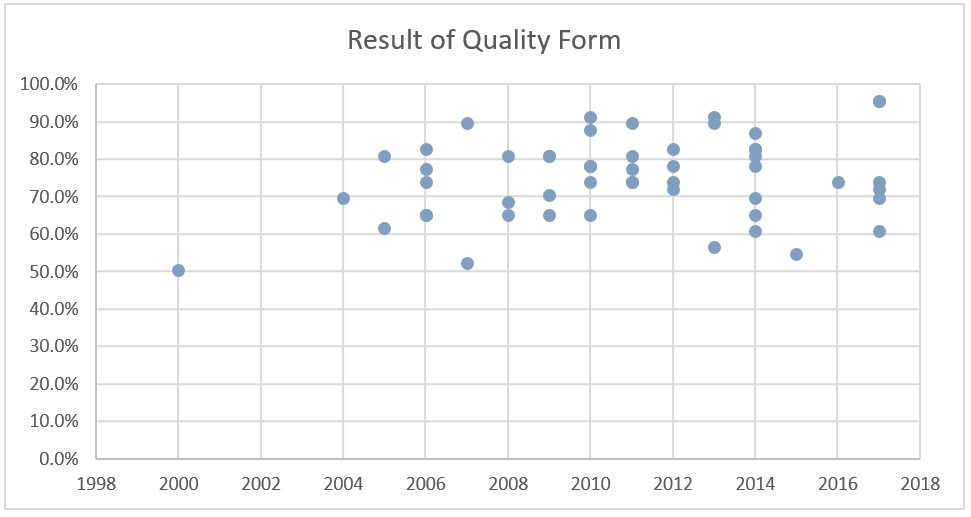
\includegraphics[width=16cm]{figuras/quality_form_of_papers.jpg}
		}{
			\Fonte{Produced by the author.}
		}	
	\end{figure}

\subsection{Publication type}
\label{subsec:results-slr-publication}

Among the papers selected in third filter, 30 are conference papers, 27 are scientific journals, and one is book chapters. The main conferences where the papers selected are published are ACM SIGACCES\footnote{ (\url{https://assets18.sigaccess.org/})} with 6 papers, ICDVRAT \footnote{(\url{https://www.icdvrat.org/})} with 5 papers and UAHCI \footnote{(\url{http://2018.hci.international/uahci})} with 3 papers. The leading journal with three papers retrieved is the International Journal on Disability and Human Development \footnote{(\url{https://www.ncbi.nlm.nih.gov/labs/journals/int-j-disabil-hum-dev/})}.

\subsection{Authors}
\label{subsec:results-slr-authors}

We present an overview of the papers related to cognitive impact evaluation found and how these papers are distributed in the research groups around the world. The papers showed some main authors and institutions that use the cognitive impact evaluation in the context of this research.The authors and research groups distributions contribute to understanding how the cognitive impact evaluation has been applied around the world.

Considering the main authors as those who have more than one paper on the list, Figure \ref{fig:quality_form_of_papers2} shows tag cloud\footnote{Performed in the WordArt tool - \url{https://wordart.com/}} based on the number of papers per authors. Sánchez, J. is the author most present in the list (with 35 papers). Other authors that stand out are Merabet, Lahav, and Sáenz.

 	\begin{figure}[h] 
   	    \captionsetup{width=12cm}%Da mesma largura que a figura
		\Caption{\label{fig:quality_form_of_papers2} Author}
		\UFCfig{}{
			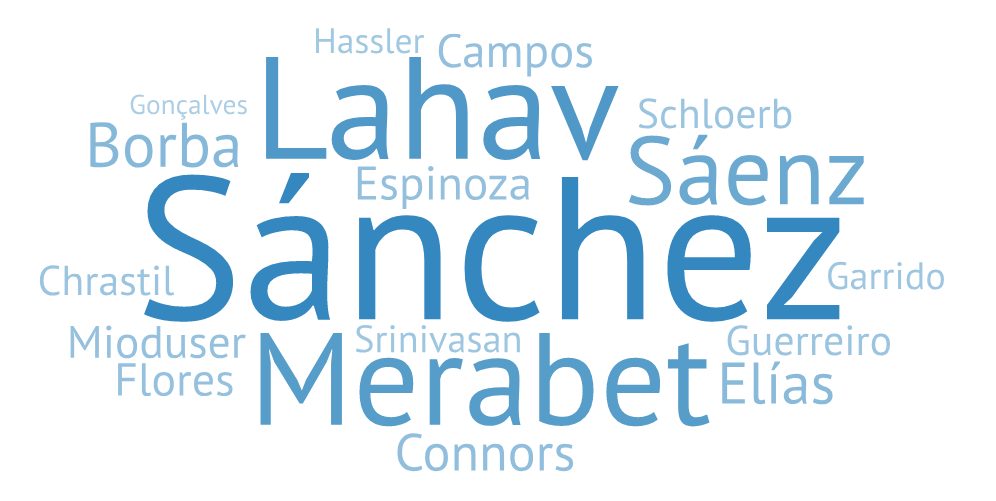
\includegraphics[width=12cm]{figuras/authors.png}
		}{
			\Fonte{Produced by the author.}
		}	
	\end{figure}

Seeking to understand better how and where these authors work, we developed an analysis based on the institutions of origin and found international research relationships between them, explained in the next session.

\textbf{Institutions around the world}

We found the author come from 42 institutions around the world. Figure \ref{fig:mapa} shows the global overview of the papers retrieved. We explore the locations by using the MAXQDA\footnote{\url{https://www.maxqda.com}} software to correlate the groups around the world. As we can see in the figure, the leading research groups in this context are in Chile, USA, and Israel. They are the Department of Computer Science at University of Chile (36 papers, 25,4\% of frequency), Laboratory for Visual Neuroplasticity at Harvard Medical School (8 papers, 5,8\%), School of Education at Tel Aviv University, Israel (7 papers, 4,8\%) and PUCRS in Brazil (4 papers).

\begin{landscape}
 	\begin{figure}[htb] 
   	    \captionsetup{width=25cm}%Da mesma largura que a figura
		\Caption{\label{fig:mapa} The global overview of the papers retrieved}
		\UFCfig{}{
			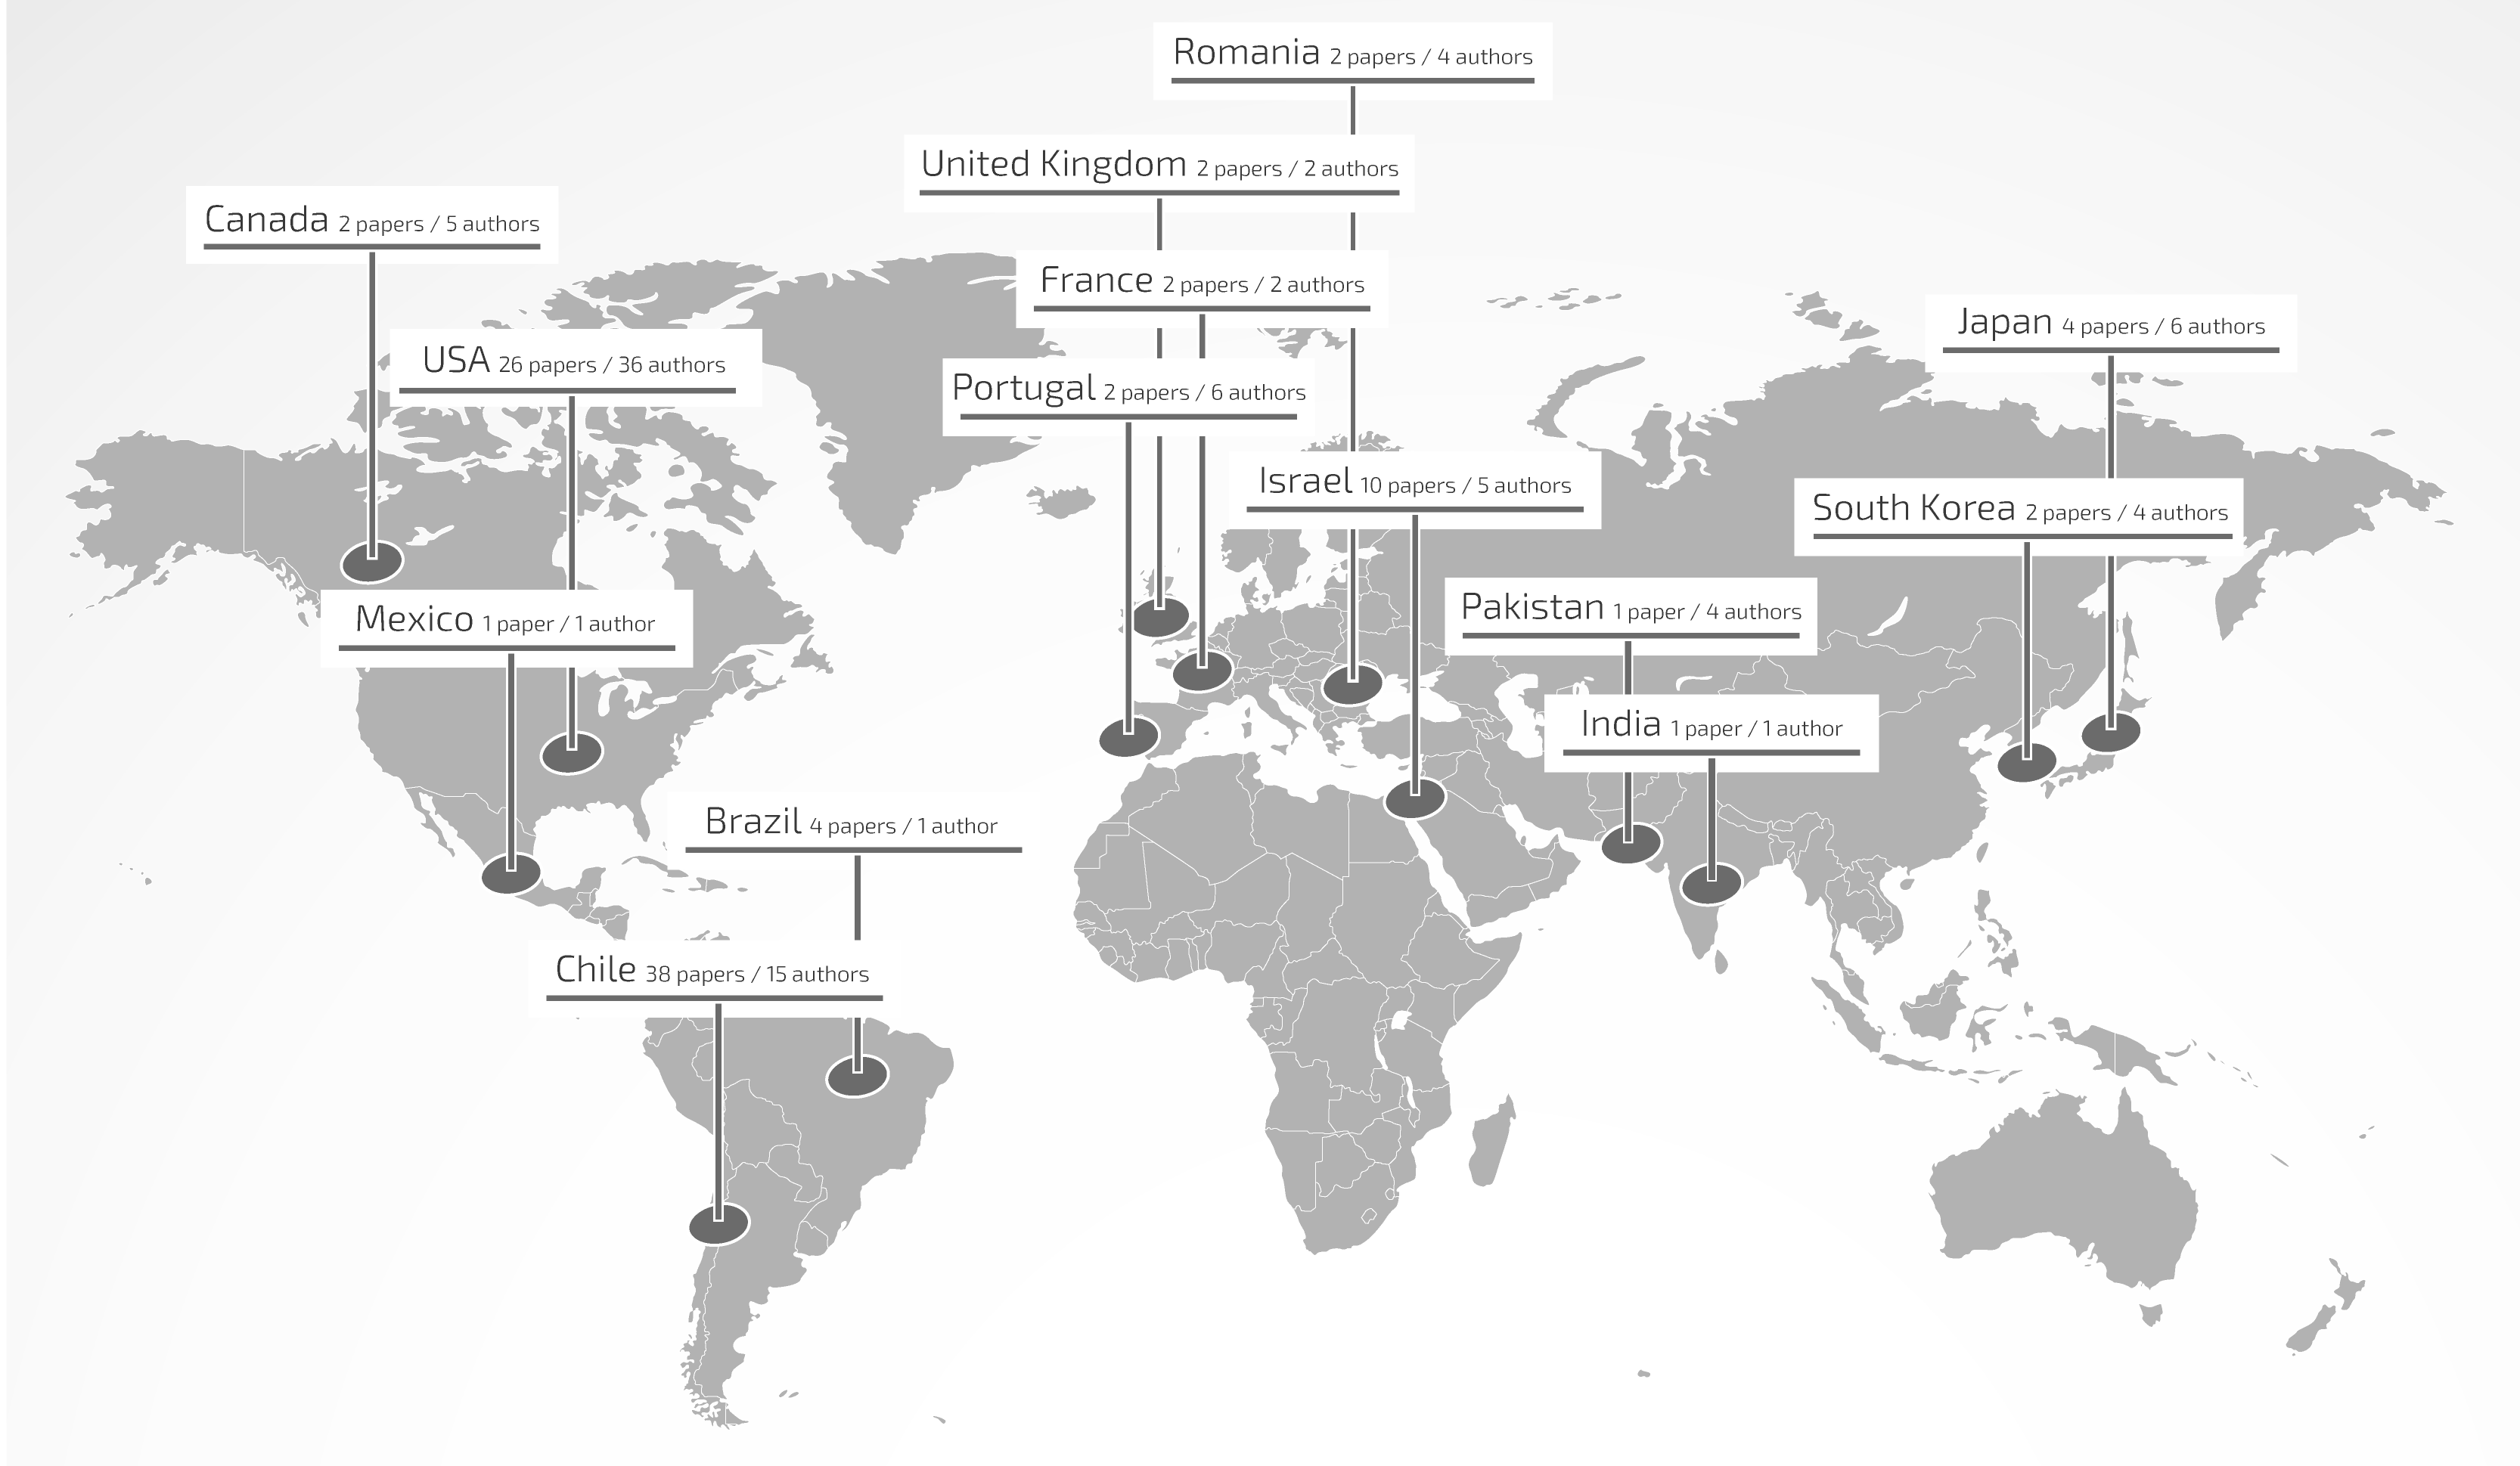
\includegraphics[width=25cm]{figuras/mapa.png}
		}{
			\Fonte{Produced by the author.}
		}	
	\end{figure}
\end{landscape}

The research cooperation between the different institutions is current practice for scientific research, and it is possible to observe in our finds. Table of the Figure \ref{fig:research_between_institutions} shows the cooperation between different institutions, even those are in the same country, as the example of Canada that has 2 institutions working together. In this data, we highlight the large number of institutions and cooperation between them from USA, Chile, and Israel. The USA has great cooperation with Chile and their research institutions. Chile also works with partnerships in Brazilian institutions. Moreover, Israel institutions also stand out by the research with their institutions and with French and American institutions.

\begin{figure}[htb] 
   	    \captionsetup{width=16cm}%Da mesma largura que a figura
		\Caption{\label{fig:research_between_institutions} Research between institutions}
		\UFCfig{}{
			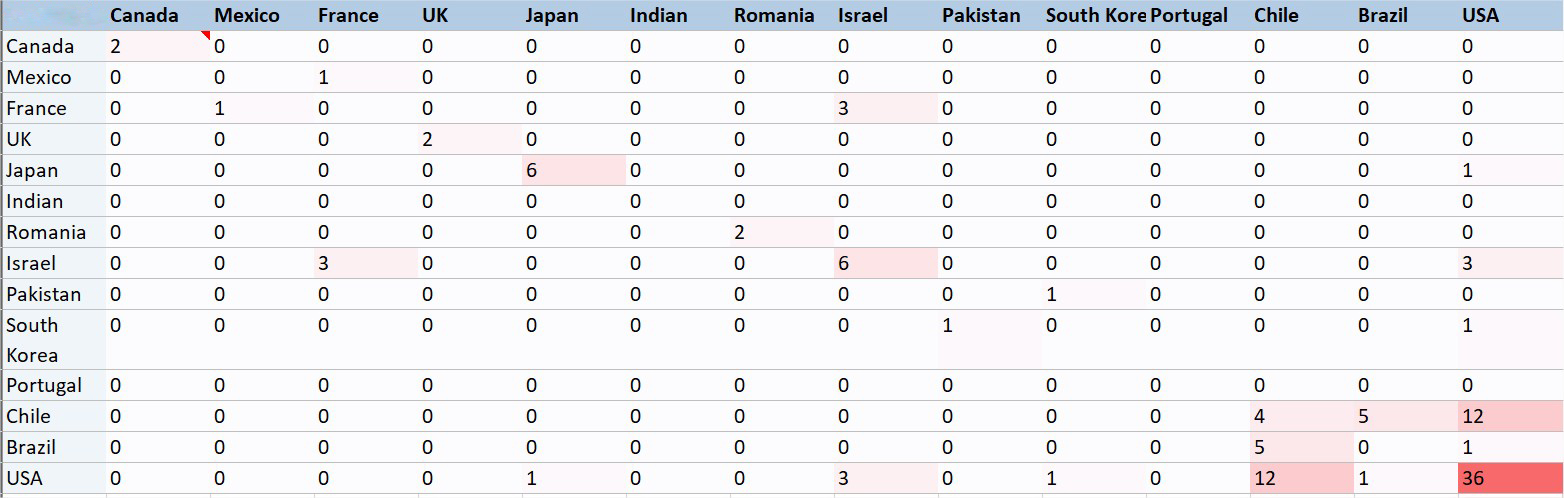
\includegraphics[width=16cm]{figuras/cooperation.jpg}
		}{
			\Fonte{Produced by the author.}
		}	
\end{figure}


%\begin{small}

%\begin{table}[h]
%	\captionsetup{width=16cm}%Deixe da mesma largura que a tabela
%	\Caption{\label{tab:research_between_institutions} Research between institutions}%
%	\IBGEtab{}{%
%		\begin{tabular}{m{1.6cm}m{.55cm}m{.55cm}m{.55cm}m{.55cm}m{.55cm}m{.55cm}m{.55cm}m{.55cm}m{.55cm}m{.55cm}m{.55cm}m{.55cm}m{.55cm}m{.55cm}}
%			\toprule
%			Cooperation System & Cana- da & Me- xico & Fran- ce & UK & Japan & In- dian & Rom- ania & Is- rael & Pakis- tan & South Korea & Portu- gal & Chi- le & Bra- zil & USA\\
			%\cellcolor[HTML]{AA0044} para dar cor a celula basta colar esse codigo antes do valor da celula.
%			\midrule \midrule
%			Canada & 2 & 0 & 0 & 0 & 0 & 0 & 0 & 0 & 0 & 0 & 0 & 0 & 0 & 0 \\
%			Mexico & 0 & 0 & 1 & 0 & 0 & 0 & 0 & 0 & 0 & 0 & 0 & 0 & 0 & 0 \\
%			France & 0 & 1 & 0 & 0 & 0 & 0 & 0 & 3 & 0 & 0 & 0 & 0 & 0 & 0 \\
%			UK & 0 &  0 & 0 & 2 & 0 & 0 & 0 & 0 & 0 & 0 & 0 & 0 & 0 & 0 \\
%			Japan & 0 & 0 & 0 & 0 & 6 & 0 & 0 & 0 & 0 & 0 & 0 & 0 & 0 & 1 \\
%			Indian & 0 & 0 & 0 & 0 & 0 & 0 & 0 & 0 & 0 & 0 & 0 & 0 & 0 & 0 \\
%			Romania & 0 & 0 & 0 & 0 & 0 & 0 & 2 & 0 & 0 & 0 & 0 & 0 & 0 & 0 \\
%			Israel & 0 & 0 & 3 & 0 & 0 & 0 & 0 & 6 & 0 & 0 & 0 & 0 & 0 & 3 \\
%			Pakistan & 0 & 0 & 0 & 0 & 0 & 0 & 0 & 0 & 0 & 1 & 0 & 0 & 0 & 0 \\
%			South Korea & 0 & 0 & 0 & 0 & 0 & 0 & 0 & 0 & 1 & 0 & 0 & 0 & 0 & 1 \\ 
%			Portugal & 0 & 0 & 0 & 0 & 0 & 0 & 0 & 0 & 0 & 0 & 0 & 0 & 0 & 0 \\
%			Chile & 0 & 0 & 0 & 0 & 0 & 0 & 0 & 0 & 0 & 0 & 0 & 4 & 5 & 12 \\
%			Brazil & 0 & 0 & 0 & 0 & 0 & 0 & 0 & 0 & 0 & 0 & 0 & 5 & 0 & 1 \\
%			USA & 0 & 0 & 0 & 0 & 1 & 0 & 0 & 3 & 0 & 1 & 0 & 12 & 1 & 36 \\
%			\bottomrule
%		\end{tabular}%
%	}{%
%	\Fonte{Autor.}%
%	\Nota{esta é uma nota, que diz que os dados são baseados na	regressão linear.}%
%	\Nota[Anotações]{uma anotação adicional, seguida de várias outras.}%
 %   }
 %   \end{table}   
%\end{small}

\subsection{Tools evaluated}
\label{subsec:results-tools}

Finally, in the general data acquired, we search to understand which kind of technology the studies present and evaluate. We search a broader view of tools, which means the tool or application should not have to be specific for people who are blind or visually impaired, but it needs to have into the technology search criteria specified in the Section \ref{subsec:methodology-conducting} and must have a cognitive impact evaluation. A non-standard example of applications found is a study that assesses the cognitive impact of an ATM machine by people who are blind. 

Some papers develop the cognitive evaluation with the same tool, thus, we detect 45 tools evaluated among papers selected. Appendix \ref{ap:A} list all tools detailed. The tools and applications were classified according to the type of activity performed into 8 categories: 
        \begin{enumerate}
            \item School learning: applications that improve school subjects such as mathematics and biology;
            \item Game: applications with gamification elements that develop cognitive characteristics;
            \item Maps: applications that works with indoor and outdoor maps whether virtual or real to develop cognitive navigation, mobility or orientation processes;
            \item Others, as objects structure learning, input text on a telephone keypad, mobile device and ATM machine.
        \end{enumerate}

Figure \ref{fig:technology_type} shows the results of classification. The applications that works with maps, mobility, orientation and navigation are the most common.

 	\begin{figure}[h] 
   	    \captionsetup{width=12cm}%Da mesma largura que a figura
		\Caption{\label{fig:technology_type} Technology type}
		\UFCfig{}{
			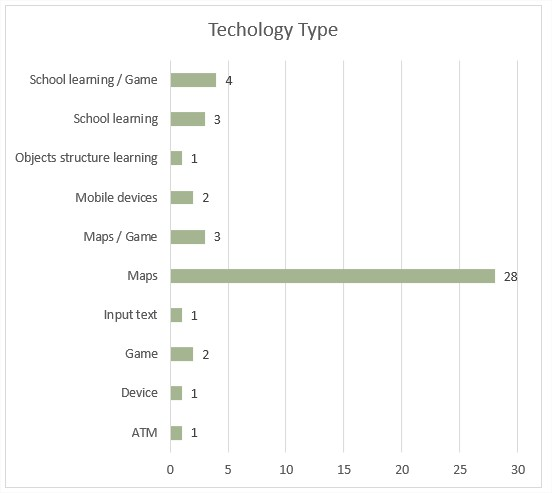
\includegraphics[width=12cm]{figuras/technology_type.jpg}
		}{
			\Fonte{Produced by the author.}
		}	
	\end{figure}

\section{Research results}
\label{sec:results-research}
This category aims to understand the focus of each paper regarding the research done. First, we present others strategies of the technology evaluation encountered in the selected papers. 

\subsection{Other Strategies of the evaluation applied}
\label{subsec:results-other-strategies}

Many papers apply another approach to evaluate other criteria not covered in our study, as shown in Figure \ref{fig:other_strategies}. Usability evaluation is the most used assessment besides impact evaluation. This kind of assessment is mainly used to obtain information about the user's acceptance of the software, and the match between his or her mental model and the representation included in the software \cite{Sanchez2009a}. Others are evaluation based on HCI heuristics \cite{Shafiq2014}, iconic evaluation \cite{Sanchez2011}, recognition of patterns, obstacle awareness goal and homing and obstacle avoidance \cite{Pissaloux2017TowardsDevices}.

 	\begin{figure}[h] 
   	    \captionsetup{width=12cm}%Da mesma largura que a figura
		\Caption{\label{fig:other_strategies} Quantity of other evaluation strategies used}
		\UFCfig{}{
			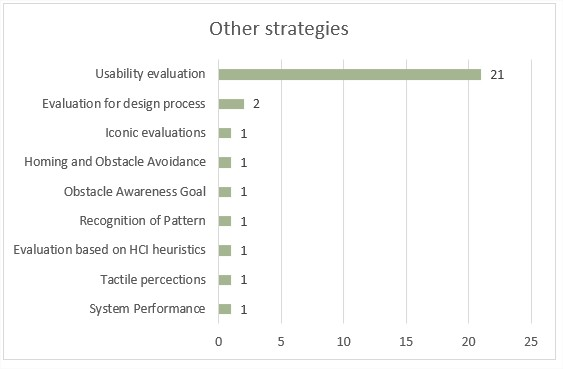
\includegraphics[width=12cm]{figuras/other_strategies.jpg}
		}{
			\Fonte{Produced by the author.}
		}	
	\end{figure}

\subsection{Classification}
\label{subsec:results-classification}

The classification of the key features in multimodal interfaces for the cognition of people who are blind proposed by \citeonline{Darin2015} is adapted to classify the papers, already presented in Figure \ref{fig:Key_features _in_multimodal_interfaces_(evaluation)}. This classification is divided into 4-dimension: Interface, Interaction, Cognition, and Evaluation; and it is applied to video games and virtual environments. These features provide necessary insights for the practical understanding of the issues involved in their design and evaluation \citeonline{Darin2015}. These features are useful in our research for giving a comprehensive overview of technologies and evaluations regarding the multimodal interfaces.

We cover, in the classification, more than video games and virtual environments since we also found these features present in the technologies selected. We did not divide the features of the evaluation domain into cognitive and usability evaluation. Instead, we focus on typical activities and instruments, which in our perception can be applied to the impact evaluations that were found. Then, the result of this classification is shown in Figure \ref{fig:key_features_evaluation}.

 %	\begin{figure}[h] 
  % 	    \captionsetup{width=16cm}%Da mesma largura que a figura
%		\Caption{\label{fig:key_features_multimodal_interfaces_results} Key features in multimodal interfaces}
%		\UFCfig{}{
%			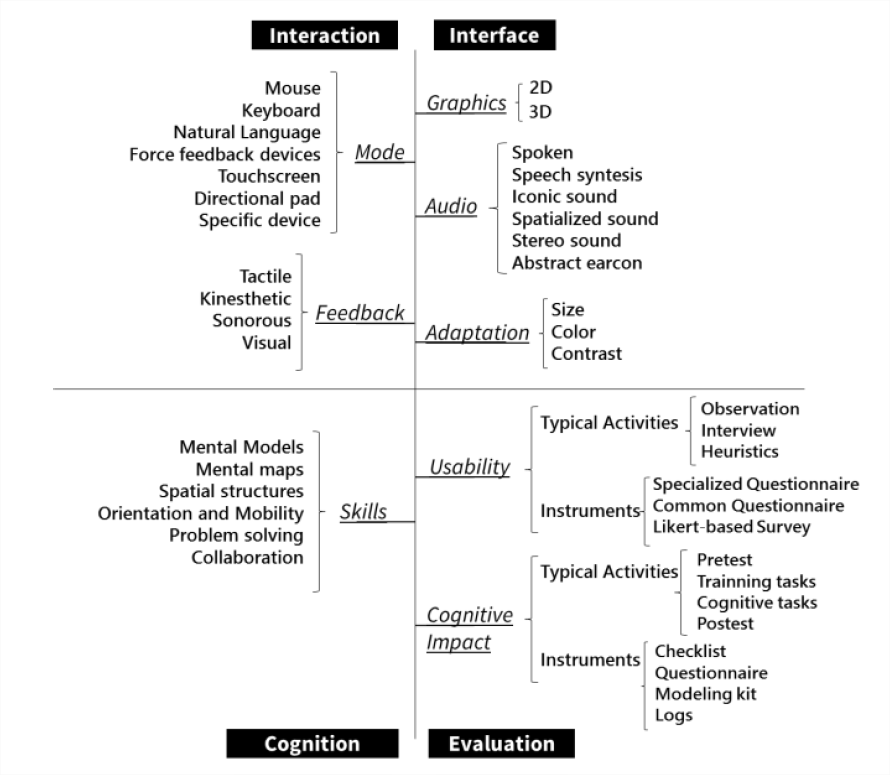
\includegraphics[width=16cm]{figuras/key_features_multimodal_interfaces.png}
%		}{
%			\Fonte{\citeonline{Darin2015}.}
%		}	
%	\end{figure}
	
 	\begin{figure}[h] 
   	    \captionsetup{width=12cm}%Da mesma largura que a figura
		\Caption{\label{fig:key_features_evaluation} Key features in multimodal interfaces (Evaluation)}
		\UFCfig{}{
			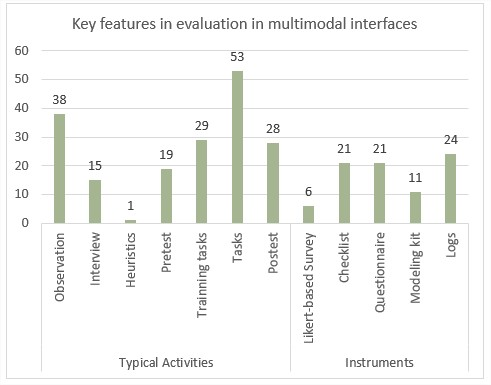
\includegraphics[width=12cm]{figuras/key_features_evaluation.jpg}
		}{
			\Fonte{Produced by the author.}
		}	
	\end{figure}


As we can see, the Keyboard is the main mode to interact with technologies analyzed. It is an instrument of interaction already common as input device \cite{Sanchez2004}. The keyboard does not generate more complexity and expenses, like the Novint Falcon device, that is used in \cite{Sanchez2014a}. The Novint Falcon is one of the Force Feedback Device that promotes a Tactile and Kinesthetic Feedback. Mouse and Natural language are less used. The mouse is replaced by buttons or other specific devices for a better interaction, as shown in \cite{Shafiq2014}. The most common Feedback is the Sonorous and the main Audio Interface used is the Iconic Sound, which are sounds associated with each available object and action in the environment \cite{Sanchez2014a}.

These characteristics are important to understand which kind of interfaces are assessed and how the impact is evaluated on them. The Evaluation dimension will be discussed in more depth in the following sections.

\section{Empirical data results}
\label{sec:results-empirical}

The Empirical category aims to answer the research question of the systematic literature review in detail. The data retrieved ground the comprehension of the main research question. Thus, we search the main aspects concerning the empirical method applied. Note, in this category, we analyze the 47 papers selected on the fourth filter that brings 52 experiments process since five papers have two different experiments. In addition to the Systematic Literature Review (SLR) method, we use the Grounded Theory method to analyze the empirical data. With this combination of methods, we construct a concept based on cognitive assessment data. Figure \ref{fig:Key_features _in_multimodal_interfaces_(evaluation)} shows the data were chosen to be retrieved and which method had been primarily used.

 	\begin{figure}[h] 
   	    \captionsetup{width=12cm}%Da mesma largura que a figura
		\Caption{\label{fig:Key_features _in_multimodal_interfaces_(evaluation)} Empirical data extracted from experiments}
		\UFCfig{}{
			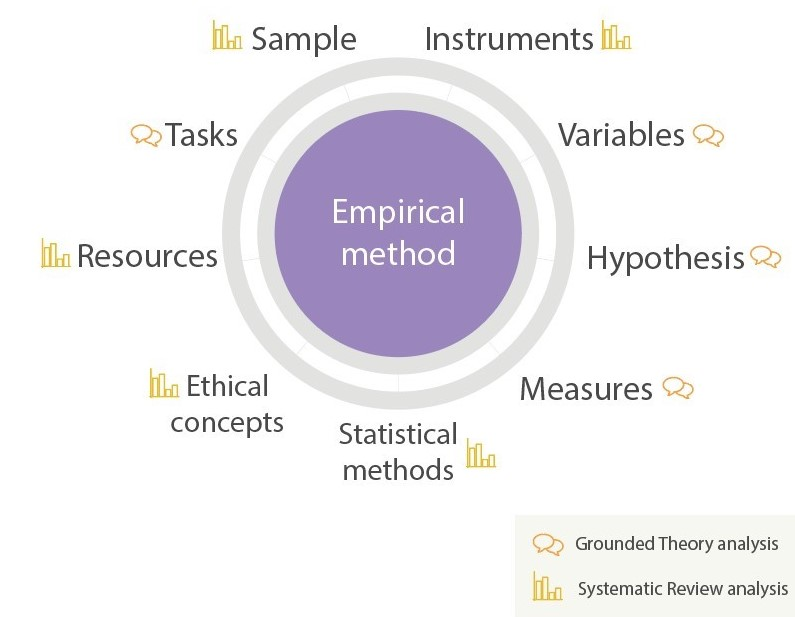
\includegraphics[width=12cm]{figuras/Key_features_in_multimodal_interfaces_(evaluation).jpg}
		}{
			\Fonte{Produced by the author.}
		}	
	\end{figure}

\subsection{Sample}
\label{subsec:results-sample}

In the sample data analysis, we look for the sampling strategy and the samples description, including the number of participants (per condition) and the kind of participants (e.g., computer science students). Figure \ref{fig:sample_information} shows the sample information retrieved from each experiment. This information is one of the main specificities of the type of experiment sought here, that is, of the cognitive evaluation of multimodal interfaces for people who are blind.
%\begin{landscape}
	\begin{figure}[h] 
       \captionsetup{width=15cm}%Da mesma largura que a figura
	\Caption{\label{fig:sample_information} Sample information}
	\UFCfig{}{
		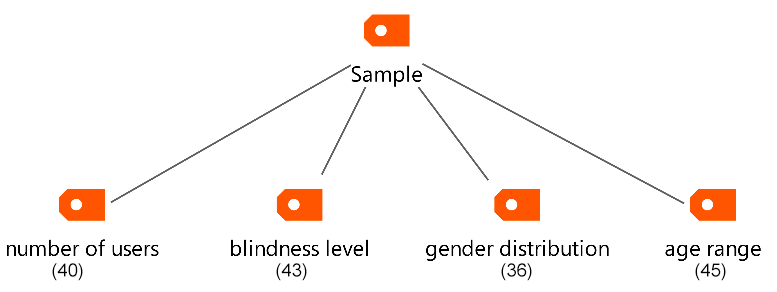
\includegraphics[width=15cm]{figuras/sample_information.png}
	}{
		\Fonte{Produced by the author.}
	}	
	\end{figure}
%\end{landscape}


\textbf{Number of users}

From the number of users to the onset age of blindness, there are many sample combinations in the selected experiments. The sample choice includes previous experience required to do the task and others characteristic controlled in the experiment, like disabilities, the onset of blindness, the etiology of a visual impairment or the presence of another disability. The quantity of users varies as shown in Figure \ref{fig:number_of_users}. Most of the experiments (22) are applied to 6 to 10 users. One experiment does not inform the number of users. One experiment \cite{Hossain2011} expresses the small number of the sample (4 blinds participants) as a limitation/implication of the research. Moreover, the paper talks about the limited access to people who are blind, and those who use a smartphone are even more difficult.

There is no guideline about the number of users on an experiment sample in the context of this research. The tradeoff between limitations and quality of the research should define the number of users. The planning phase must propose a plausible solution with the group of participants that are sought to the experiment have a reasoned result, preferably based on statistical data.

	\begin{figure}[h] 

   	    \captionsetup{width=12cm}%Da mesma largura que a figura
		\Caption{\label{fig:number_of_users} Number of users}
		\UFCfig{}{
			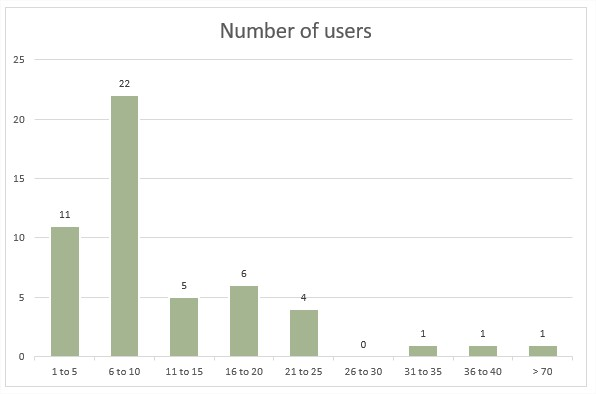
\includegraphics[width=12cm]{figuras/number_of_users.jpg}
		}{
			\Fonte{Produced by the author.}
		}	
	\end{figure}

\textbf{Gender distribution}

The gender distribution in samples is equilibrated in most cases. Figure \ref{fig:gender} shows the gender distribution on each experiment that describes how many women and men are participants (36 papers). The mean of gender proportion, among all samples, is 47\% for women and 53\% for men.

	\begin{figure}[h] 

   	    \captionsetup{width=16cm}%Da mesma largura que a figura
		\Caption{\label{fig:gender} Gender distribution}
		\UFCfig{}{
			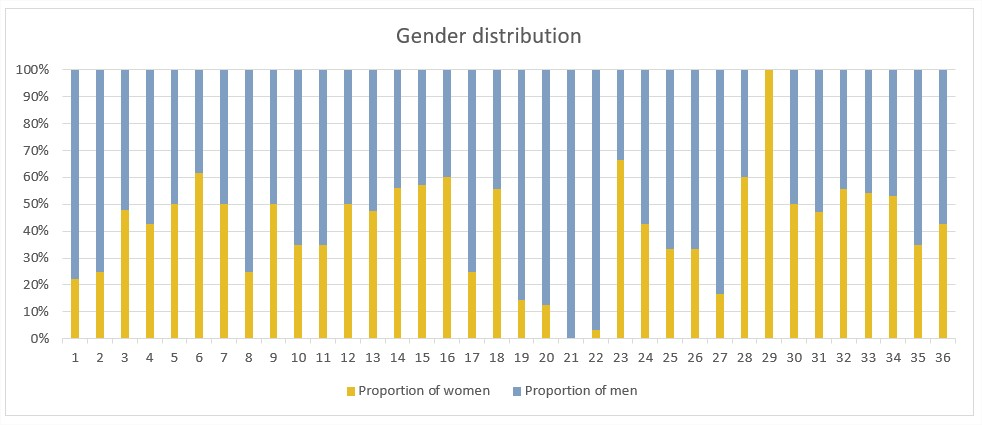
\includegraphics[width=16cm]{figuras/gender.jpg}
		}{
			\Fonte{Produced by the author.}
		}	
	\end{figure}

\textbf{Age range}

The rage of age varies a lot among the experiments. Figure 1\ref{fig:age_range} shows for each experiment the age range (green bar) and the mean (yellow line). To find a pattern, we adopted age groups based on indications of the Brazilian Child and Adolescent Statute (ECA) \cite{CasaCivil1990EstatutoAdolescente} and the Brazilian Statute of the Elderly \cite{CasaCivil2003EstatutoIdoso}, which defines 4groups: child (under age12), adolescent (between age 12 and under 21) , adult (between age 21 and 59) and elderly (over 60 years old). Figure \ref{fig:age_range_2} shows the distribution among age groups. The most of experiments (20 experiments) are applied in adults. 7 experiments do not inform the age of participants.

	\begin{figure}[h] 

   	    \captionsetup{width=16cm}%Da mesma largura que a figura
		\Caption{\label{fig:age_range} Age range of users}
		\UFCfig{}{
			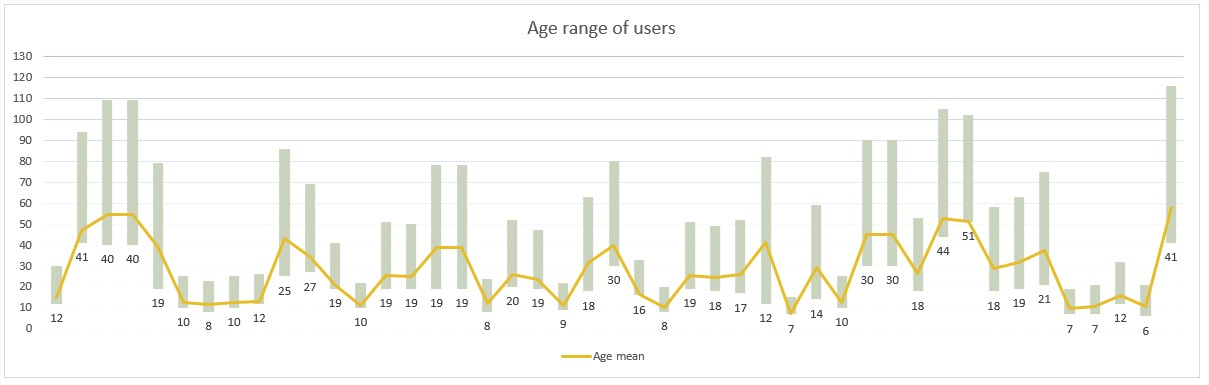
\includegraphics[width=16cm]{figuras/age_range.jpg}
		}{
			\Fonte{Produced by the author.}
		}	
	\end{figure}

	\begin{figure}[h] 

   	    \captionsetup{width=12cm}%Da mesma largura que a figura
		\Caption{\label{fig:age_range_2} Age distribution by groups}
		\UFCfig{}{
			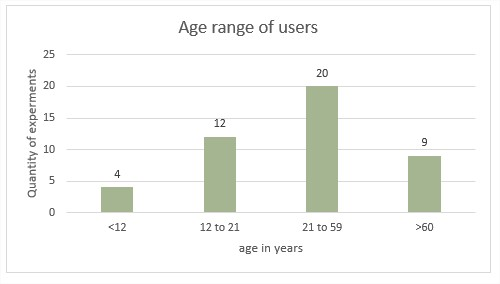
\includegraphics[width=12cm]{figuras/age_range_2.jpg}
		}{
			\Fonte{Produced by the author.}
		}	
	\end{figure}

\textbf{Blindness level}

%%%%Comentário do .doc%%%%%%%%%
%%%Explorar mais a importância desta informação, da seleção desse número e citar os pontos fora da curva: 
%18 artigos só tem pessoas cegas 
%1 artigo só tem pessoas videntes (explicar pq esse entrou) 
%4 artigos utilizam blindfolded --- citar artigo que explica pq não é bom usar blindfolded
%falar ainda de outras informações sobre o nível de cegueira, como onset, origem, tempo, se nasceu ou se se tornou ao longo da vida, se possui outras deficiências... 
%além disso informar, se possível, o nível de cegueira na escala apresentada na fundamentação teórica
%%%

The distribution between the blindness level is varied. There are experiments where the sample is all formed by people who are blind \cite{Lahav2012,Sanchez2005c}, and there are samples formed only by people who are blindfolded, as the experiments in \cite{Pissaloux2017TowardsDevices}. Table \ref{tab:blindproportion} shows the blindness level distribution between the samples. Although it is essential information in the context of the experiments studied here, 9 experiments do not inform the proportions of blind, low vision, sighted and blindfolded. 
\begin{comment}

%%% Tabela excluida e comentada %%%
\begin{table}[h]
	\captionsetup{width=14cm}%Deixe da mesma largura que a tabela
	\Caption{\label{tab:blindproportion} Kind of Instruments}%
	\IBGEtab{}{%
		\begin{tabular}{m{3cm}m{3.5cm}m{3cm}m{3cm}}
			\toprule
		    Proportion of blind & Proportion of low vision & Proportion of Sighted & Proportion of blindfolded \\
			\midrule \midrule
			100\% & 0\% & 0\% & 0\% \\
			100\% & 0\% & 0\% & 0\% \\
			100\% & 0\% & 0\% & 0\% \\
			100\% & 0\% & 0\% & 0\% \\
			100\% & 0\% & 0\% & 0\% \\
			100\% & 0\% & 0\% & 0\% \\
			100\% & 0\% & 0\% & 0\% \\
			100\% & 0\% & 0\% & 0\% \\
			100\% & 0\% & 0\% & 0\% \\
			100\% & 0\% & 0\% & 0\% \\
			100\% & 0\% & 0\% & 0\% \\
			100\% & 0\% & 0\% & 0\% \\
			100\% & 0\% & 0\% & 0\% \\
			100\% & 0\% & 0\% & 0\% \\
			100\% & 0\% & 0\% & 0\% \\
			100\% & 0\% & 0\% & 0\% \\
			100\% & 0\% & 0\% & 0\% \\
			100\% & 0\% & 0\% & 0\% \\
			93\% & 7\% & 0\% & 0\% \\
			80\% & 20\% & 0\% & 0\% \\
			80\% & 20\% & 0\% & 0\% \\
			75\% & 25\% & 0\% & 0\% \\
			75\% & 25\% & 0\% & 0\% \\
			67\% & 33\% & 0\% & 0\% \\
			56\% & 44\% & 0\% & 0\% \\
			53\% & 47\% & 0\% & 0\% \\
			52\% & 48\% & 0\% & 0\% \\
			51\% & 3\% & 44\% & 0\% \\
			50\% & 50\% & 0\% & 0\% \\
			50\% & 0\% & 0\% & 50\% \\
			50\% & 0\% & 0\% & 50\% \\
			44\% & 56\% & 0\% & 0\% \\
			43\% & 57\% & 0\% & 0\% \\
			35\% & 65\% & 0\% & 0\% \\
			33\% & 67\% & 0\% & 0\% \\
			29\% & 71\% & 0\% & 0\% \\
			25\% & 75\% & 0\% & 0\% \\
			25\% & 38\% & 38\% & 0\% \\
			22\% & 0\% & 0\% & 78\% \\
			22\% & 0\% & 0\% & 78\% \\
			20\% & 80\% & 0\% & 0\% \\
			0\% & 100\% & 0\% & 0\% \\
			0\% & 0\% & 100\% & 0\% \\
			\bottomrule 
		\end{tabular}%
	}{%
	\Fonte{Produced by the author.}%
%	\Nota{esta é uma nota, que diz que os dados são baseados na	regressão linear.}%
%	\Nota[Anotações]{uma anotação adicional, seguida de várias outras.}%
    }
    \end{table}
\end{comment}


%\begin{comment}
	\begin{figure}[h] 

   	    \captionsetup{width=16cm}%Da mesma largura que a figura
		\Caption{\label{tab:Kind_of_Instruments} Proportion of blindness level}
		\UFCfig{}{
			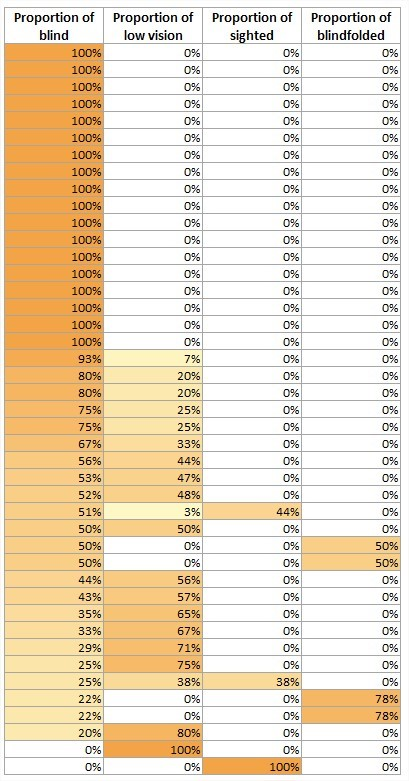
\includegraphics[width=10cm]{figuras/kind_of_instruments.jpg}
		}{
			\Fonte{Produced by the author.}
		}	
	\end{figure}
%\end{comment}

\subsection{Instruments}
\label{subsec:results-instruments}

The instruments used in the evaluation has the objective to identify some user ability controlled on the Experiment (as an independent variable), e.g., the mathematics knowledge test in \citeonline{Sanchez2005,Sanchez2005c} or is used to guide the evaluation process, e.g., observation guideline to assess O\&M skills in \citeonline{Sanchez2011}. 37 experiments described the instruments used. Among the instruments used, there are 5 Likert-based surveys, 20 checklists (which include guidelines and specific tests), 15 questionnaires (which include surveys), 8 modeling kits (which are manual instruments, as pen and papers or bricks), and 9 logs (which include, in addition to the system log, the video and audio logs). None instrument has been used in more than one study experiment from our list. We speculate this is due to the distinct natures of skills evaluated. Figure \ref{fig:kind} shows the ethical concepts retrieved.

	\begin{figure}[h] 

   	    \captionsetup{width=12cm}%Da mesma largura que a figura
		\Caption{\label{fig:kind} Type of Instruments}
		\UFCfig{}{
			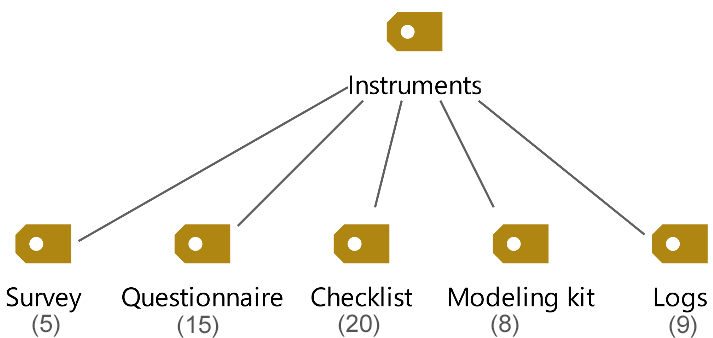
\includegraphics[width=12cm]{figuras/kind.png}
		}{
			\Fonte{Produced by the author.}
		}	
	\end{figure}

\subsection{Statistical Methods}
\label{subsec:results-statistical-methods}

Figure \ref{fig:statistical_methods} shows the statistical methods used in the experiment data analysis. We do not take account of the common statistical methods, like averages and gain percent. In 3 experiments, the statistical method was not described or explicit in the text, neither in the references. T-test, which uses statistical concepts to reject or not a null hypothesis, is the most used, followed by ANOVA and Person’s Correlation, that is used to analyze the variation between groups. ANOVA procedure was applied in one, two and three-way. 

	\begin{figure}[h] 

   	    \captionsetup{width=16cm}%Da mesma largura que a figura
		\Caption{\label{fig:statistical_methods} Statistical methods}
		\UFCfig{}{
			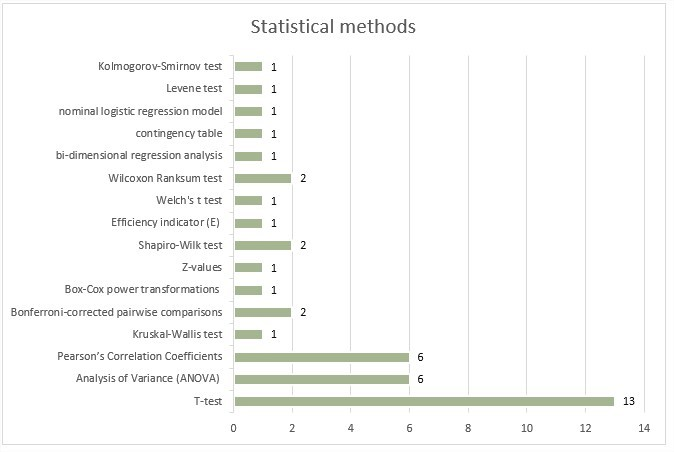
\includegraphics[width=16cm]{figuras/statistical_methods.jpg}
		}{
			\Fonte{Produced by the author.}
		}	
	\end{figure}

The statistical method used depends on the research goal and the data acquired of the experiment. Thus, we prefer not to present the methods according to the type of analysis, such as hypothesis analysis or correlation between variables. Instead, we focused on if the experiment data analysis has any statistical method applied. Our objective is not to discuss how to apply the best method, but to analyze the evidence based on statistical confirmations. However Figure \ref{fig:statistical_type} presents the two types of use to the statistical methods.

	\begin{figure}[h] 

   	    \captionsetup{width=12cm}%Da mesma largura que a figura
		\Caption{\label{fig:statistical_type} Statistical type}
		\UFCfig{}{
			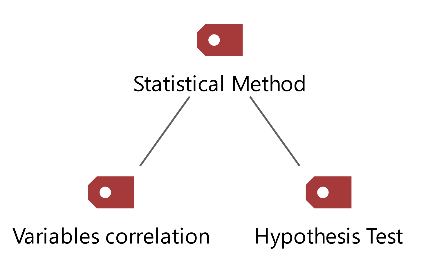
\includegraphics[width=12cm]{figuras/statistical_type.png}
		}{
			\Fonte{Produced by the author.}
		}	
	\end{figure}

\subsection{Resource data}
\label{subsec:results-resource-data}

In general, the papers do not present resource data of the experiments in the text. 19 experiments describe some information about the resource, as time-period, costs or human resources. Among this information, the time-period presented varies from 2 days to 6 months with the mean of 3 months-period. 4 experiments explain some information about cost, two of them chose some technology due to their low cost. One experiment says pay \$25 per hour to participants, and another pays \$60 for 3-hour sessions. One paper describes their team to apply the experiment. Almost always there is little or no information about the resources, this can hinder the replication of the experiment, as well as it lacks evidence to the descriptive text about adequacy, limits, qualities, costs and associated risks. Figure \ref{fig:resource_information} shows the resource information retrieved.


	\begin{figure}[h] 

   	    \captionsetup{width=12cm}%Da mesma largura que a figura
		\Caption{\label{fig:resource_information} Resource information}
		\UFCfig{}{
			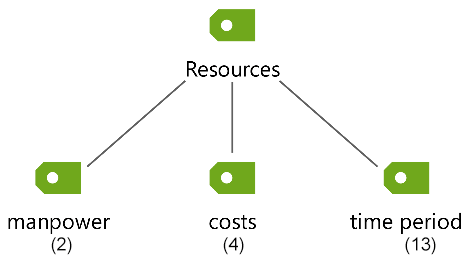
\includegraphics[width=12cm]{figuras/resource_information.png}
		}{
			\Fonte{Produced by the author.}
		}	
	\end{figure}

\subsection{Ethical Concepts}
\label{subsec:results-ethical-concepts}


The ethical concepts also are not well covered in the papers; even it is an essential step to produce an experiment with people who have disabilities \cite{Wohlin2000}. Among papers that threats the ethical concepts, 8 papers mentioned signing consents, two of them also applies to stop rules to enforcing ethical concept; 6 papers present the ethics council approved by legal institutions; two experiments express some information concern the user safety. It should be considered the local laws of ethical concepts and also the published year for each experiments. Figure \ref{fig:ethical_information} shows the sample information retrieved from each experiment. 

	\begin{figure}[h] 

   	    \captionsetup{width=12cm}%Da mesma largura que a figura
		\Caption{\label{fig:ethical_information} Ethical concepts}
		\UFCfig{}{
			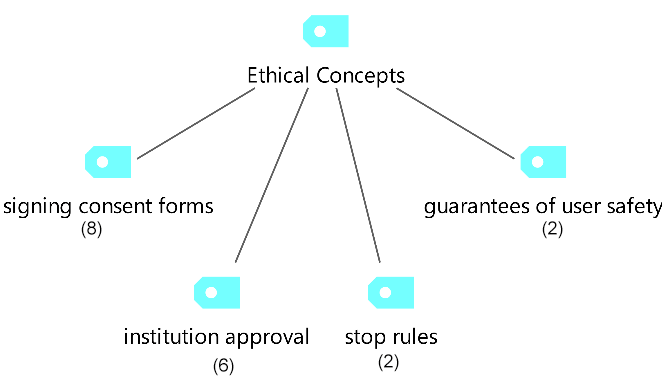
\includegraphics[width=12cm]{figuras/ethical_information.png}
		}{
			\Fonte{Produced by the author.}
		}	
	\end{figure}



\subsection{Hypothesis and groups}
\label{subsec:results-hypothesis}

Hypothesis is the basis for the statistical analysis of an experiment. A hypothesis is stated formally, and the data collected during the experiment is used to, if possible, reject the hypothesis \cite{Wohlin2000}. If the hypothesis can be rejected, then conclusions can be drawn, based on the hypothesis testing under given risks \cite{Wohlin2000}. Thus, the hypothesis is the core of the experiment design. Seeking to understand the hypothesis, we select which experiments have explicit in the text the Hypothesis and which of them test it. Even if the paper explains the research question or the goal of the experiment in the text, we do not count these. Wohlin divides the Hypothesis formulation from the Goal definition as two different phases of the experiment process. 

Figure \ref{fig:hypothesis} shows the two codes derived from this category. The ``Hypothesis well explicit'' is coded when the paper presents the hypothesis structured very well, as the experiments from ``Model of Cognitive Mobility for Visually Impaired'' \cite{Pissaloux2017TowardsDevices}.

	\begin{figure}[h] 

   	    \captionsetup{width=6cm}%Da mesma largura que a figura
		\Caption{\label{fig:hypothesis} Hypothesis}
		\UFCfig{}{
			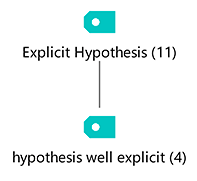
\includegraphics[width=6cm]{figuras/hypothesis.png}
		}{
			\Fonte{Produced by the author.}
		}	
	\end{figure}
	
\subsection{Variables}
\label{subsec:results-variables}

Almost no paper presents the variables explicitly in the text as dependent variables and independent variables. Thus, along with the text, we look for these variables to understand how the experiment is designed. After the grounded theory process, we produce three categories of dependent variables and three categories of independent variables. In searching this, we can see the variables are strongly related to the experiment hypothesis or objective when the hypotheses are not explicit in the text. As a result, Figure \ref{fig:variables__code_map} presents the code map generated and next we explain each variable structure.
\begin{landscape}
     	\begin{figure}[h] 

   	    \captionsetup{width=25cm}%Da mesma largura que a figura
		\Caption{\label{fig:variables__code_map} Variables code map}
		\UFCfig{}{
			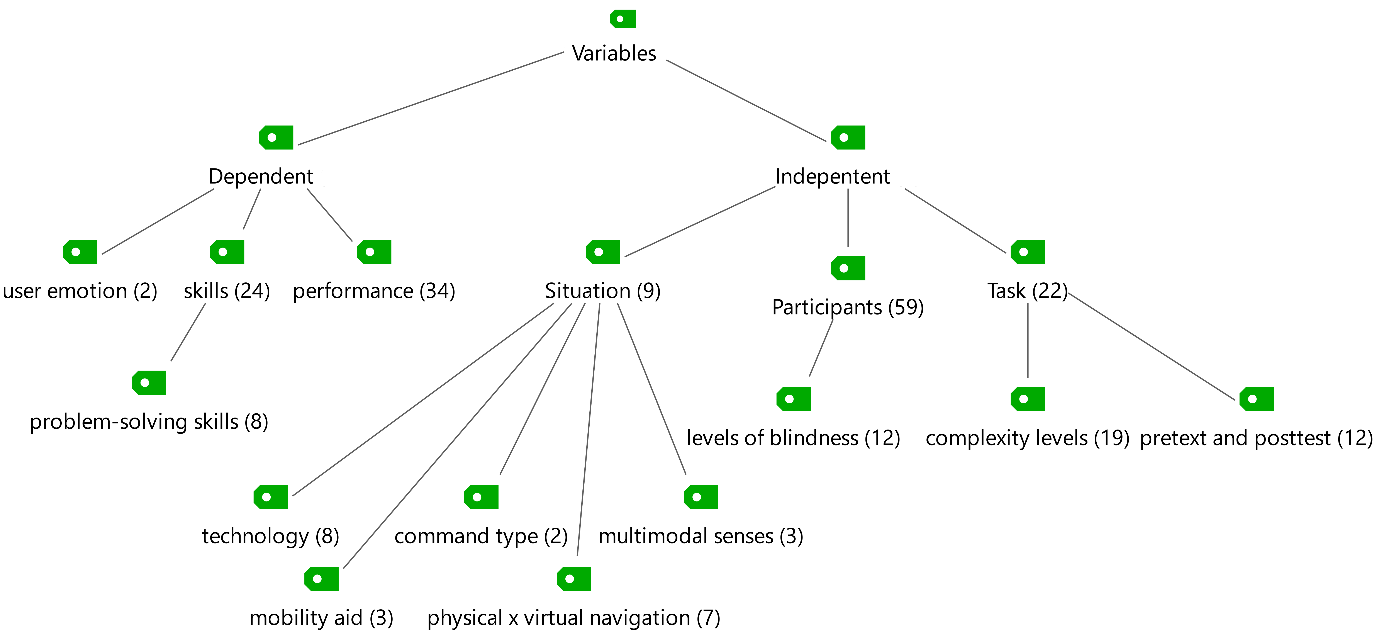
\includegraphics[width=25cm]{figuras/variables__code_map.png}
		}{
			\Fonte{Produced by the author.}
		}	
	\end{figure}
\end{landscape}

Dependent variables depend on how one or more independent variables influence or affect the participants in the experiment \cite{Wohlin2000}. As cognitive impact evaluation, the dependent variable is related to cognition processes. The main category of dependent variables is the task performance that has many ways to measure (explored in the Section \ref{subsec:results-measures}). We code as skills all dependent variables that work with a cognitive skill affected by some independent variable. Problem-solving skill stands out in the experiments and it turned a branching of skill. In the context, problem-solving, that can be understood as the act of consciously apply rules and procedures to bridge the gap between the initial problem state and a solution state \cite{Glatzeder2010}, involves solving, tasks and issues related to the application to users who are blind. Only two papers use some user emotion, as user opinion.

The independent variables are those variables that we can control and change in the experiment \cite{Wohlin2000}. So, they are related to domain knowledge. The independent variables encountered are characteristics of the situation, the participants and the tasks. The code map shows the categories that stand out in the data. Generally, the characteristics of the situation and tasks are factors, while participants characteristic are variables controlled, as etiology of blindness or age of participants. Nevertheless, usually, the levels of blindness are factors in the experiments used to divide the sample into groups \cite{Lee2014,Sanchez2000}.

Beyond the independent and dependent variables, we encountered in the grounded data other topics about the variables. 11 experiments have their variables well described in a separated section in the text. 8 experiments work with a control group to compare with the treatment. Also, three experiments stand out concern about the confounding variables. Report these topics shows more rigor in the controlled experiments, moreover it is not a usual practice.

\subsection{Tasks}
\label{subsec:results-tasks}

The tasks explored in the experiments are related to the technology assessed. Figure \ref{fig:tasks_code_map} shows the categories grounded in the experiment data. The two main categories are: Maps and Problem-Solving, this last was already discussed in the Variables section (Section \ref{subsec:results-variables}). As we have already presented in Section Technology, 31 experiments work with maps applications that aims to develop O\&M skills and other skills related. Not all presented in detail the tasks and measures, but we divide the Maps category into: \textit{(i)} location (indoor or outdoor maps), \textit{(ii)} number of spaces (one or more spaces), \textit{(iii)} known spaces (new or public spaces), \textit{(iv)} type (virtual or real map tasks), \textit{(v)} tasks that the participant need to reproduce a map using some modeling kit, as bricks, and \textit{(vi)} tasks that use the clock \cite{SanchezVideogaming}. Note, the same task of the experiment could have more than one code. 
\begin{landscape}
    \begin{figure}[h] 

   	    \captionsetup{width=25cm}%Da mesma largura que a figura
		\Caption{\label{fig:tasks_code_map} Tasks code map}
		\UFCfig{}{
			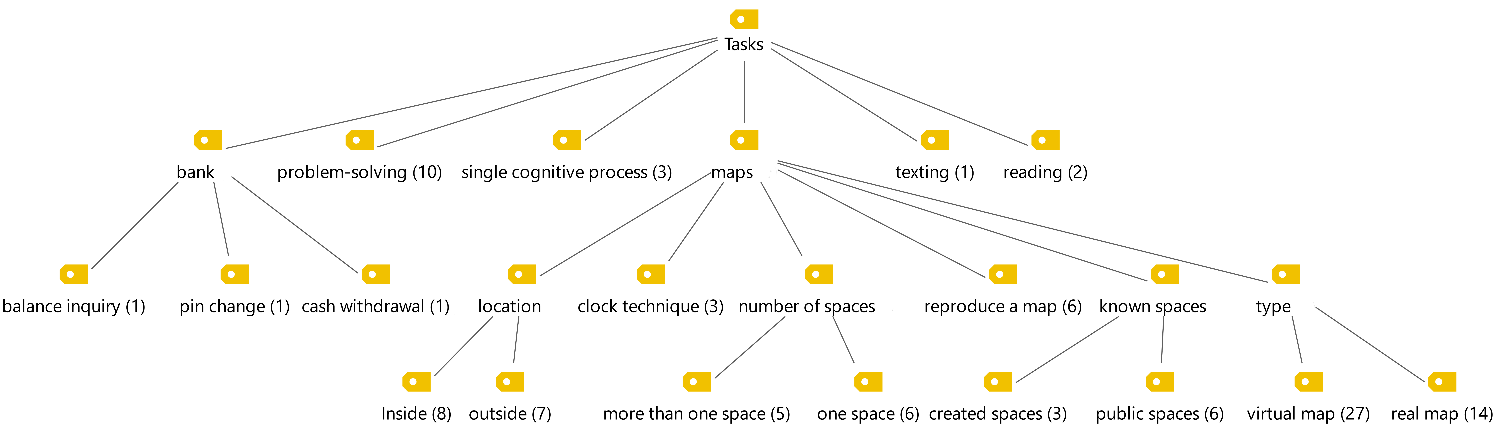
\includegraphics[width=25cm]{figuras/tasks_code_map.png}
		}{
			\Fonte{Produced by the author.}
		}	
	\end{figure}
\end{landscape}
	
\subsection{Measures}
\label{subsec:results-measures}

The measures are defined according to the variables of the experiment. Figure \ref{fig:measures_code_map} shows the Measures code map grounded in data of the experiments. We find five categories, that are measures based on \textit{(i)} technology, \textit{(ii)} activity type, \textit{(iii)} tests, \textit{(iv)} user behavior, and \textit{(v)} task performance. The categories ``activity type'' and "task performance" highlight in front of the others because they are the most used. The ``activity type'' depends on the technology domain and the variables defined. For example, one measure defined to a map task is the obstacle detection \cite{Merabet2016}. The task performance measures are the most important cognitive measures because they can be used in several domains, for example, time duration and error rate.

\begin{landscape}
	\begin{figure}[h] 

       \captionsetup{width=25cm}%Da mesma largura que a figura
	\Caption{\label{fig:measures_code_map} Measure code map}
	\UFCfig{}{
		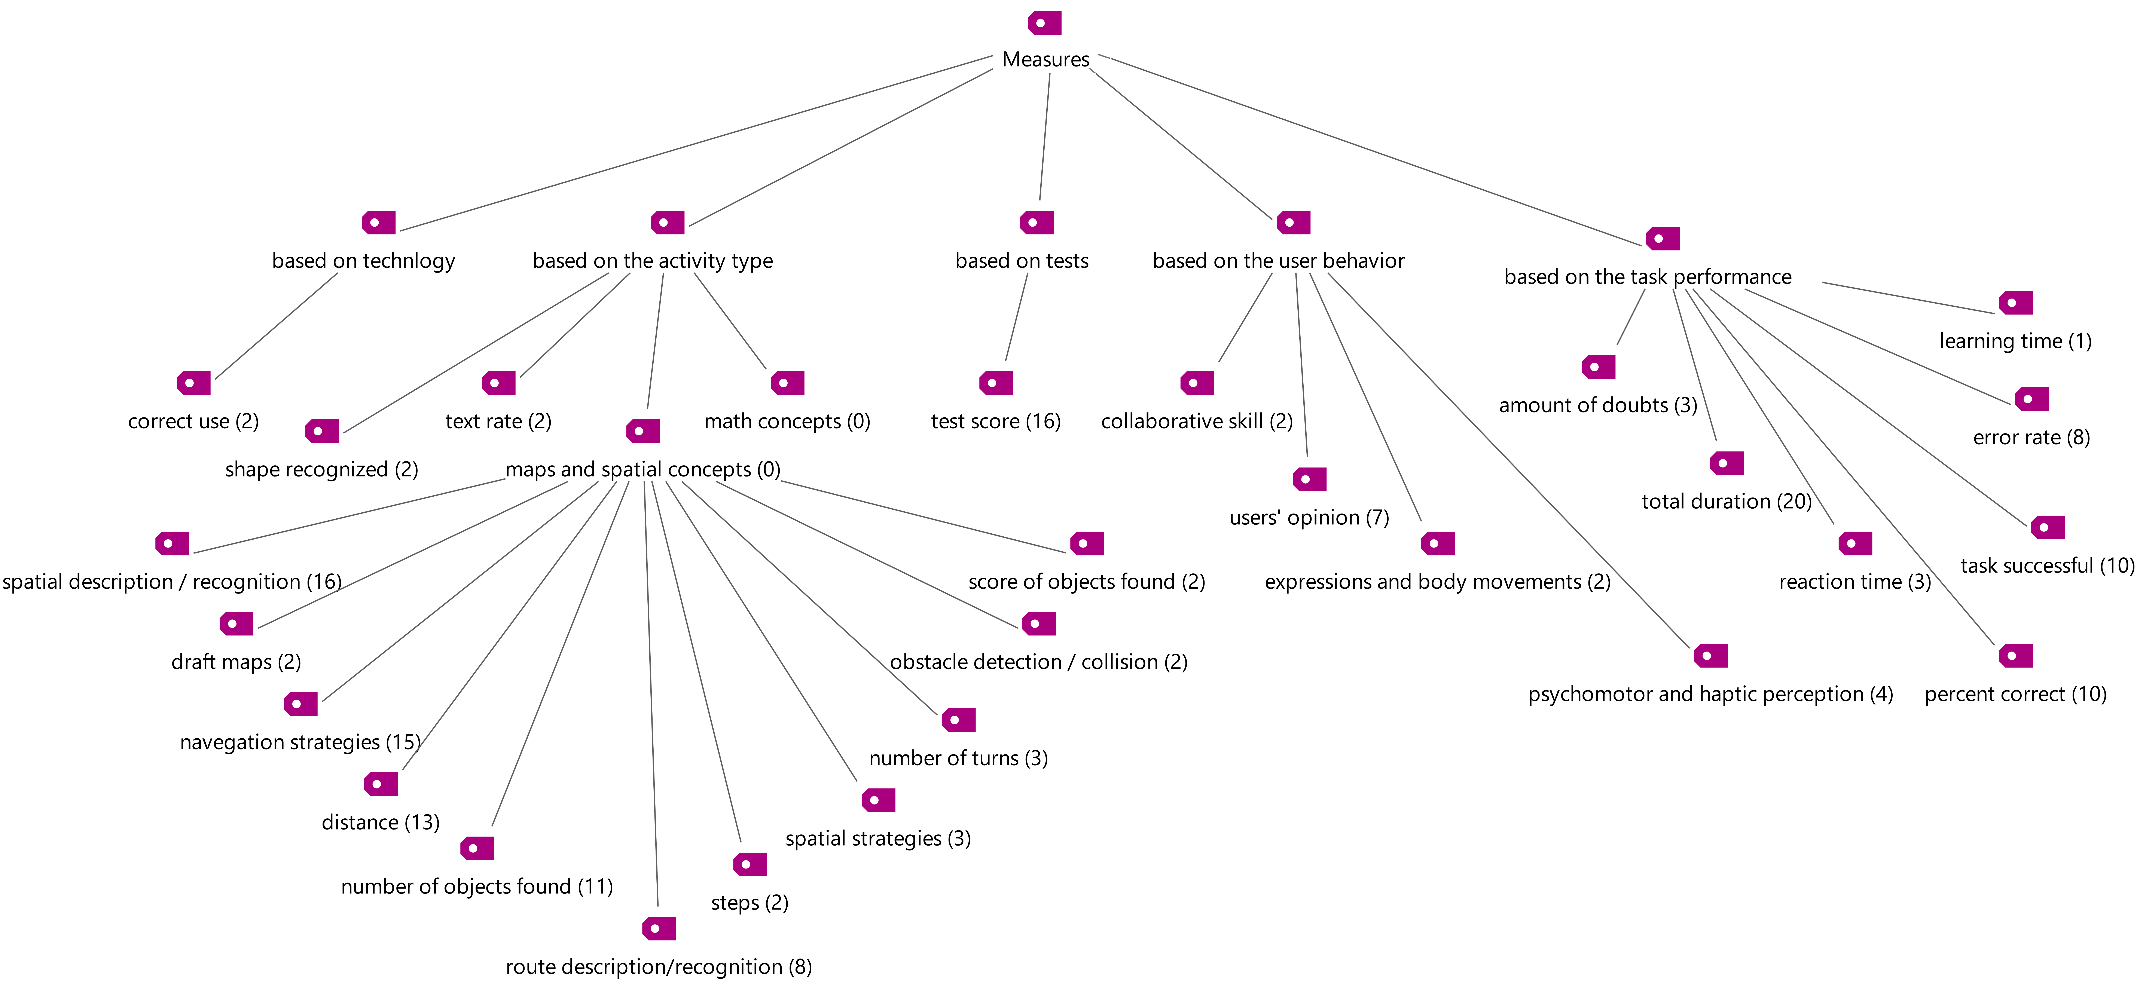
\includegraphics[width=25cm]{figuras/measures_code_map.png}
	}{
		\Fonte{Produced by the author.}
	}	
	\end{figure}
\end{landscape}

\section{Theory of Cognitive Impact Evaluation}
\label{sec:results-theory}

After organizing the core category and related the concepts of Cognitive Impact Evaluation, the data was arranged to observe the excerpts related to each concept. The relations found were identified by analyzing patterns and implicit meaning between codes. Once the concepts are related they were organized into a theoretical framework \cite{Corbin1998}, meaning the representation of concepts, together with their definitions and relations among them. Figure \ref{fig:central_idea_of_cognitive_impact} presents the cognitive impact evaluation central idea, considering the context of multimodal interfaces for people who are blind or visually impaired.

	\begin{figure}[h] 

   	    \captionsetup{width=16cm}%Da mesma largura que a figura
		\Caption{\label{fig:central_idea_of_cognitive_impact} Central idea of cognitive impact evaluation for blind users}
		\UFCfig{}{
			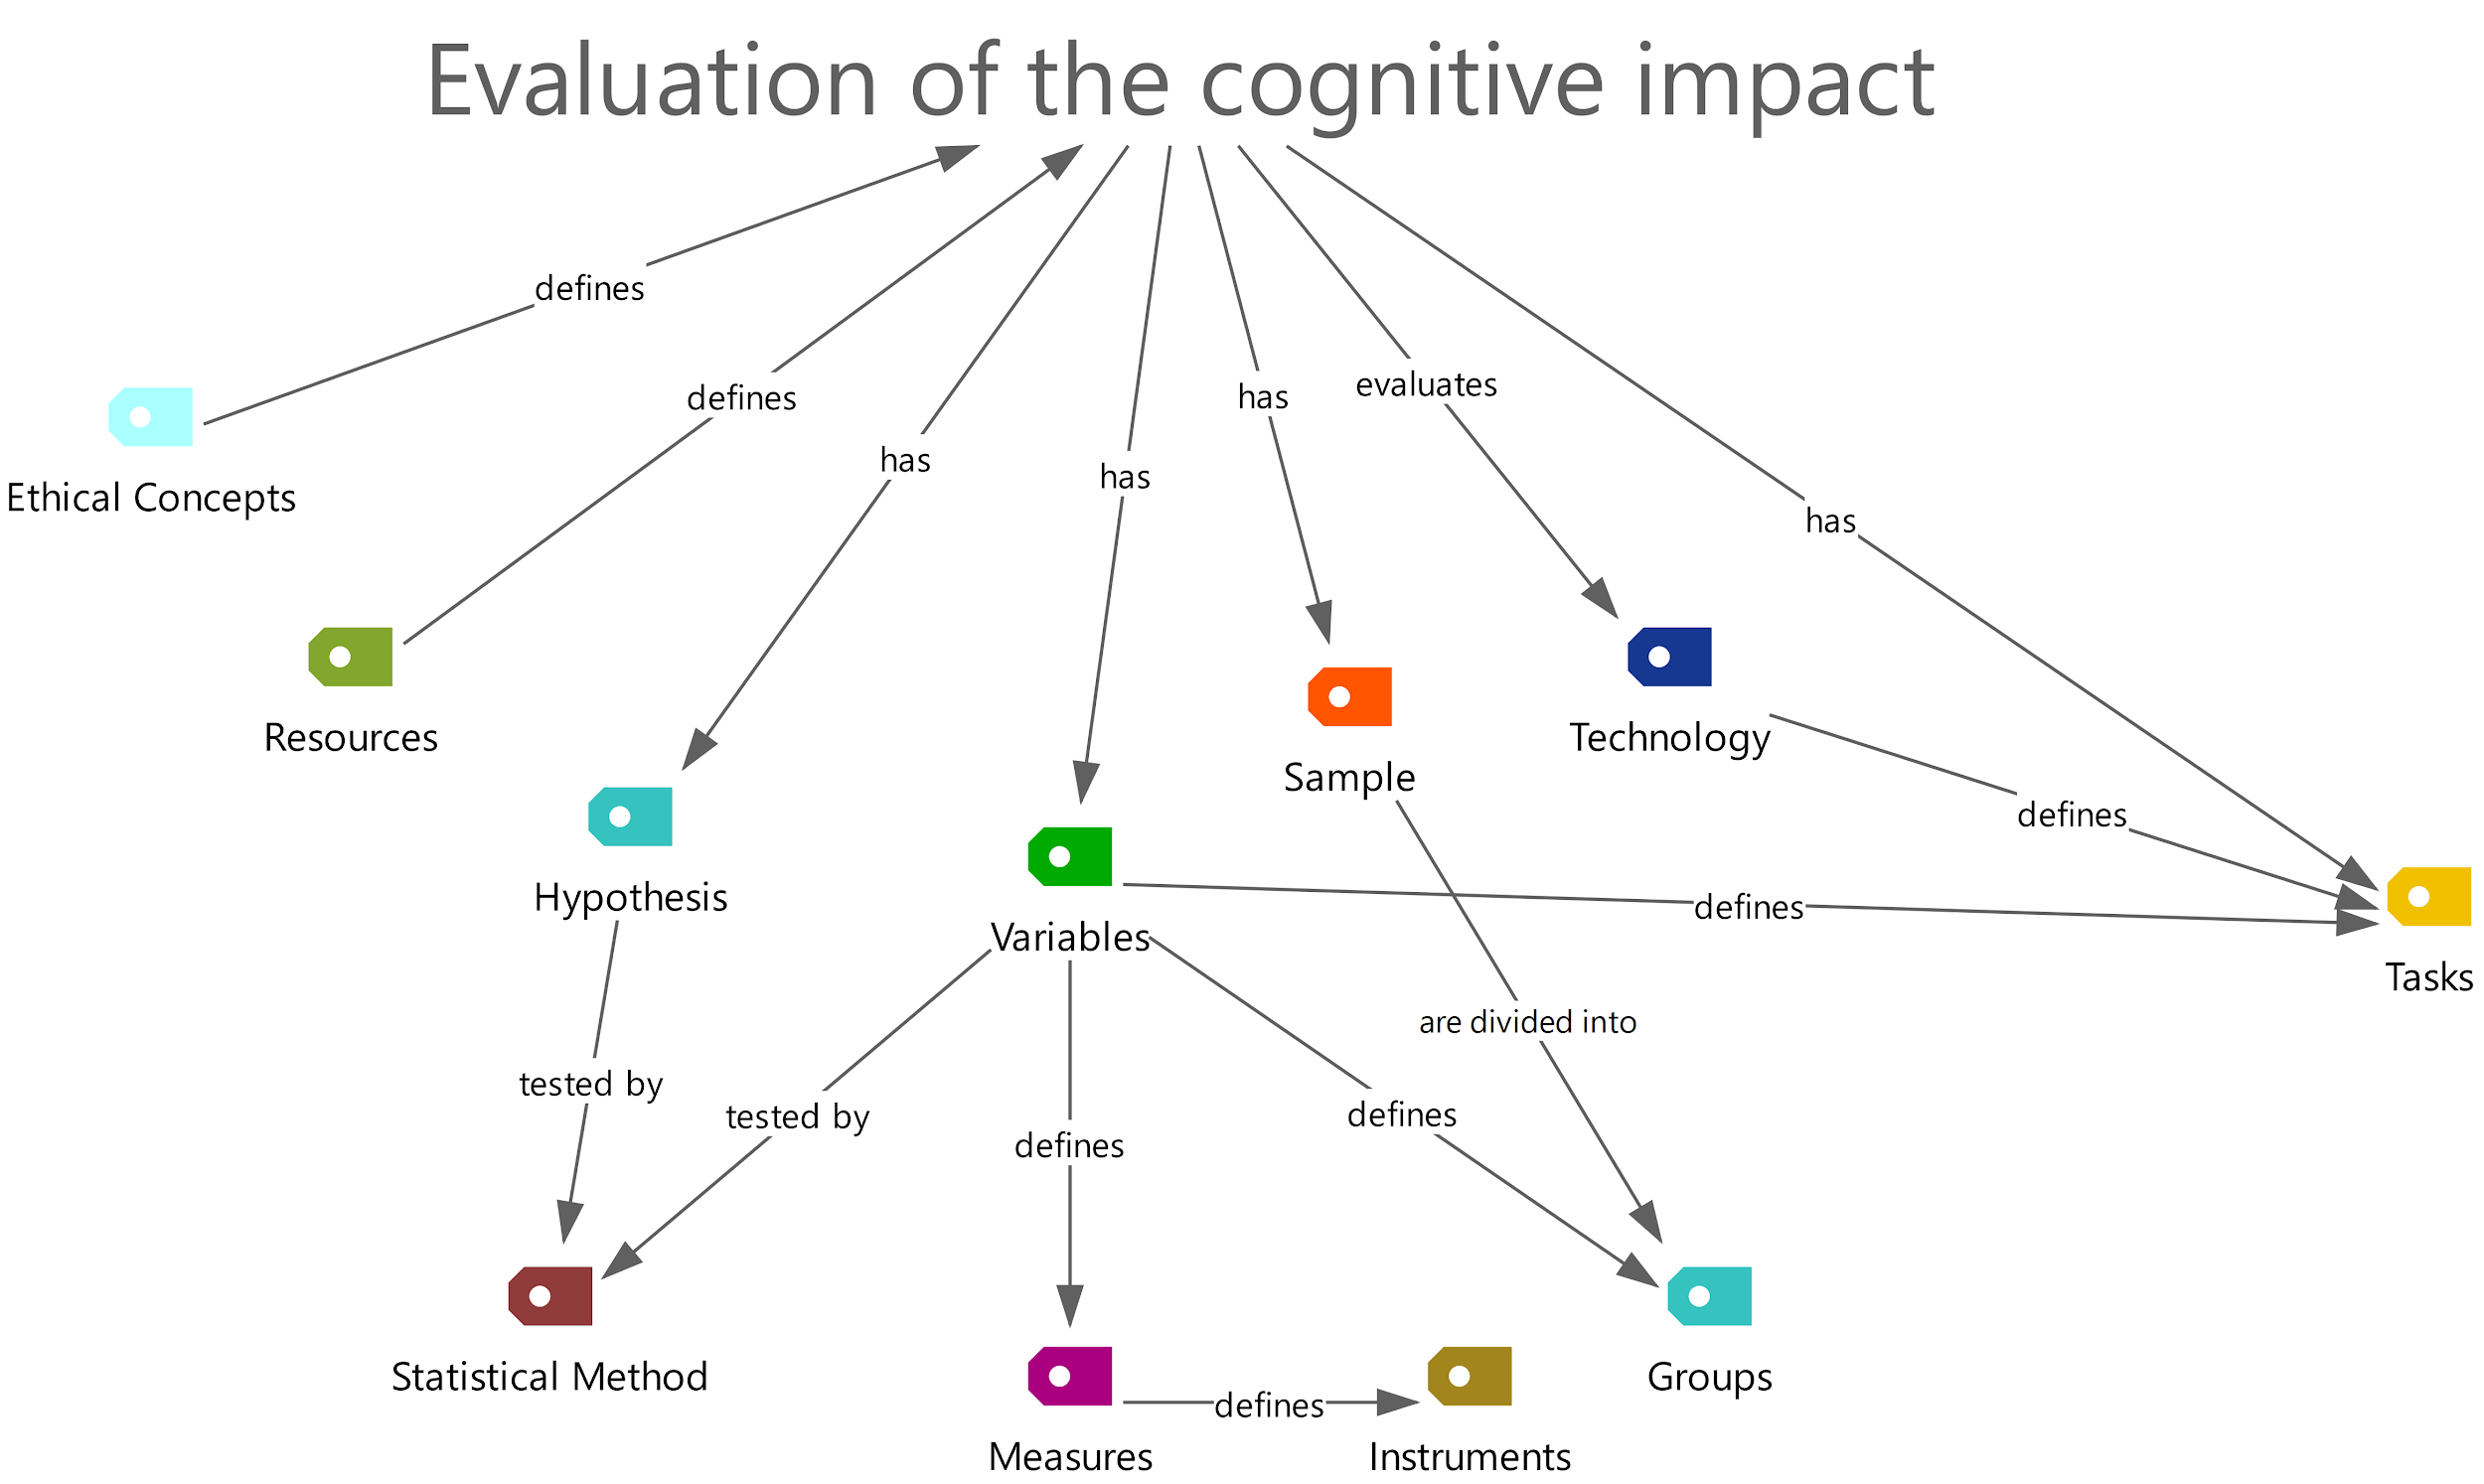
\includegraphics[width=16cm]{figuras/central_idea_of_cognitive_impact.png}
		}{
			\Fonte{Produced by the author.}
		}	
	\end{figure}
